\documentclass[12pt]{article}

\usepackage{float}
\usepackage{fancyhdr}
\usepackage{amsmath}
\usepackage{amsthm}
\usepackage{mathrsfs}
\usepackage{graphicx}
\usepackage{graphics}
\usepackage{subcaption}
\usepackage{hyperref}
\usepackage{wrapfig}
\usepackage{arydshln}
\usepackage{multirow} 
\usepackage{appendix}
\usepackage{pythonhighlight}
\usepackage{tikz}

\usepackage[natbib=true,
    style=numeric,
    sorting=none]{biblatex}
\addbibresource{bibi.bib}

\begin{document}
\begin{titlepage}
	\centering
	{\textsc{University of Bonn} \par}
	\vspace{1cm}
	{\Large \textsc{Lab report}\par}
	\vspace{1.5cm}
	{\huge\bfseries  E207: Lab Course Accelerator Bonn 
            \\(LAB)\par}
	\vspace{2cm}
	{\Large\itshape Wajdee Chayeb \\
	MohammadReza Torkamani\par}
	\vfill
	Tutor:\par
	Dr. Michael Switka

	\vfill

% Bottom of the page
	{\large \today\par}
\end{titlepage}

\tableofcontents

\section{Abstract}


Lab Accelerator Bonn (LAB) is a linear accelerator designed by ELSA staff \cite{elsa}. It has an electron gun capable of providing electrons with a kinetic energy of 25 keV. The main aim of this experiment is measuring the beam emittance of the beam emitted by the electron source. This is mainly done using two methods: Quadrupole scan and Multiscreen Method. We start our experiment by calibrating the system and aligning the beam. Then, the beam emittance is quantified in different ways and potential error sources are discussed. All information in this report is based on the lab manual \cite{lecturenote}. Therefore, any non-cited information is assumed to be taken from the manual. 

\section{LAB Experimental Setup}
Figure \ref{lab} shows a schematic illustration of the setup of LAB where the electron beam propagates from left to right. This setup consists of 4 main modules. The first module has an electron gun, two solenoids, and a corrector magnet.  The following two modules are identical and both consist of a screen, a quadrupole magnet, and a corrector magnet. Screens are used to monitor the beam profile and are thus located in front of the quadrupole magnet in each module. Finally, the last module has a mounted screen. The main objectives of elements composing the LAB setup will be explained in the next subsections.

\begin{figure}[H]
    \centering
    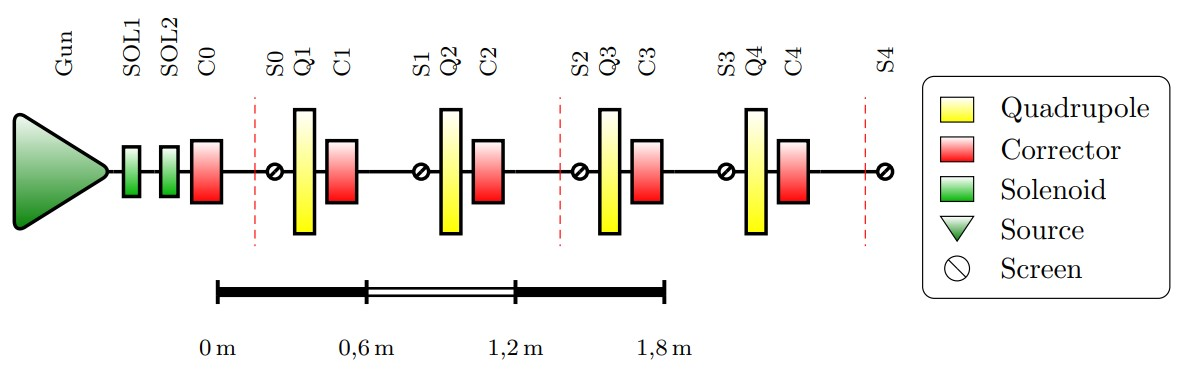
\includegraphics[width = \textwidth]{fig/LAB.jpg}
    \caption{Schematic View of the accelerator beamline \cite{lecturenote}}.
    \label{lab}
\end{figure}

\subsection*{Electron Gun}
Used to generate free electrons by heating a filament such that free electrons gain a kinetic energy high enough to overcome the binding energy and leave the material. A schematic view of the main components and potentials of the electron gun is shown in Figure \ref{electron gun}. Due to isotropic emission from the filament, an acceleration voltage of 10 V to 180 V between the filament and the cathode is applied. Then, the emitted electrons are accelerated through a potential difference of 25 kV applied between the cathode and the anode. The cathode is set to a high voltage of -25kV while the rest of the beam line including the anode is grounded. 

\begin{figure}[H]
    \centering
    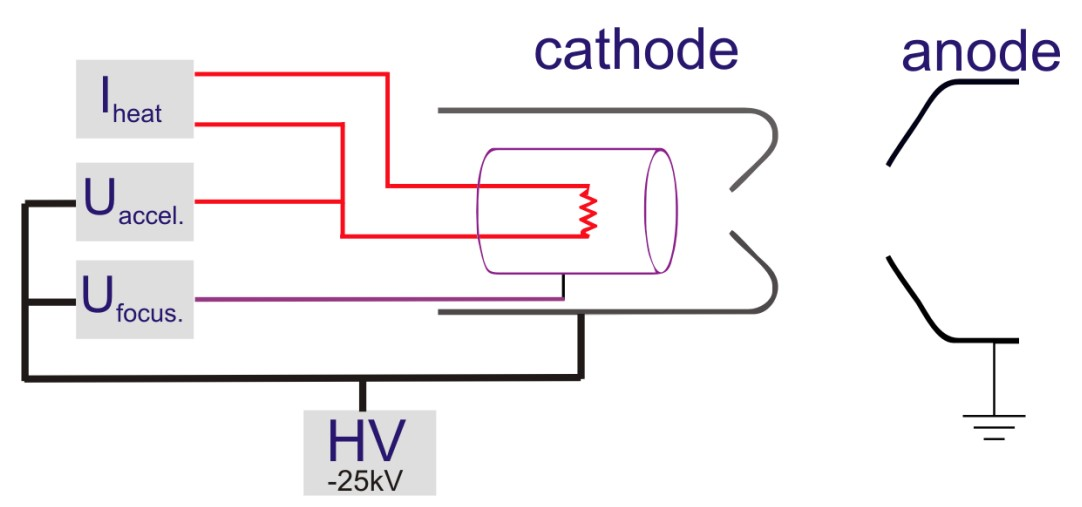
\includegraphics[width = 0.7\textwidth]{fig/electron gun.jpg}
    \caption{Schematic View of the used electron gun \cite{lecturenote}.}
    \label{electron gun}
\end{figure}


\subsection*{Solenoids}
Solenoids, which are cylindrical coils, generate a homogenous magnetic field parallel to the beam axis. This allows electrons with a transverse velocity component to be focused and deflected by fringe fields. 

\subsection*{Corrector Magnets}
Two coil pairs in a Helmholtz configuration aligned perpendicularly to the particle trajectory form a corrector magnet. This is used to move the beam trajectory to the center of quadrupole magnets where the quadrupole magnet focuses the beam only, it changes the angle of the beam trajectory by the usage of Lorentz force. A correction is needed to compensate for the deflection arising from the influence of Earth magnetic field or possible misalignment of optical elements from manufacturing imperfections.  
The deflection angle introduced by the corrector, for small angles, is expressed as:
\begin{equation}
    \alpha \simeq \frac{eBL}{p}
\end{equation}

Where e is the elementary charge of an electron, B is the magnetic field of the corrector, p is the momentum of an electron, and L is the effective length of the corrector field. 
\subsection*{Quadrupoles}
Quadrupoles used in the setup consist of four hyperbolic magnetic poles (two north poles and two south poles), as shown in Figure \ref{quadrupole}. The choice of the shape of a pole ensures a vanishing magnetic field in the center and a constant magnetic field gradient in the transverse direction. As shown in Figure \ref{quadrupole}, Lorentz force deflects electrons such that they are focused in one direction and defocused in the other. Thus, one quadrupole is not enough to get an overall focusing system. Instead, a pair of focusing and defocusing quadrupoles is used (strong focusing). 
A strength of quadrupole focusing, known as quadrupole strength, is expressed as:

\begin{equation}
    k = \frac{e}{p} g
\end{equation}

Where $k$ is the quadrupole strength, $e$ is the electric charge of an electron, p is the momentum of an electron, and $g$ is the magnetic field gradient. With the latter being constant $g = \frac{\partial B_x}{\partial z} = \frac{\partial B_z}{\partial x} = const$, a beam entering the quadrupole not in the center will have a kick angle introduced by the non-vanishing magnetic field. This effect will be used to align the electrons beam. Furthermore, the strength can also be expressed in terms of the applied current as:
\begin{equation}
    k = (128027 \pm 150) \cdot \frac{I}{p}
\end{equation}
Where $I$ is the applied current and $p$ is the electron momentum. Thus, we can change the strength by alternating the applied current. 

similar to optical lenses, a focal lens can be expressed as:
\begin{equation}
    f = \frac{1}{kL}
\end{equation}
Where $k$ is the quadrupole strength and $L$ is the effective length of the quadrupole. 



\begin{figure}[H]
    \centering
    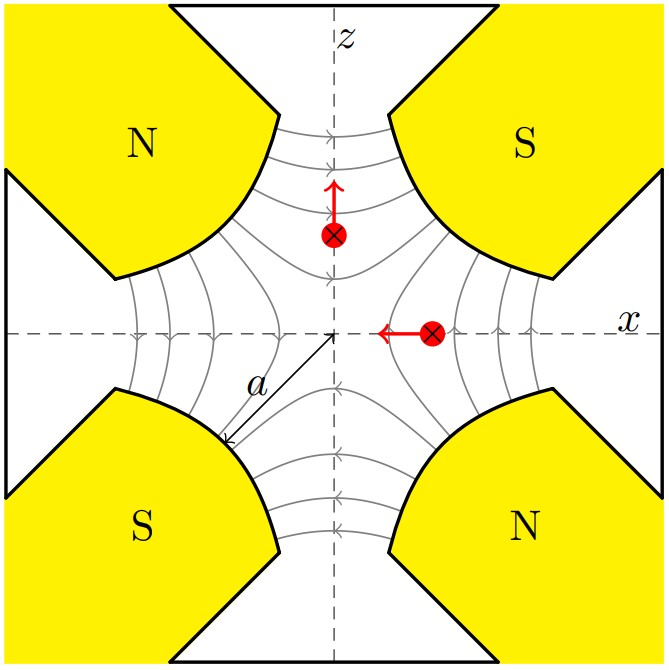
\includegraphics[width = 0.4\textwidth]{fig/quadrupole.jpg}
    \caption{Schematic view of the used quadrupole. Magnetic field lines are drawn in grey while the red dots represent electrons and the arrows indicate the direction of the Lorentz force \cite{lecturenote}.}
    \label{quadrupole}
\end{figure}

\subsection*{Screens}
To monitor the beam across different modules, screens are used. These screens are inserted into the beamline by pressurized air using a piston. Once the beam hits a screen, fluorescence light is emitted and observed at a photodiode. An illustration of a scheme of a screen is shown in Figure \ref{screen}. 

\begin{figure}[H]
    \centering
    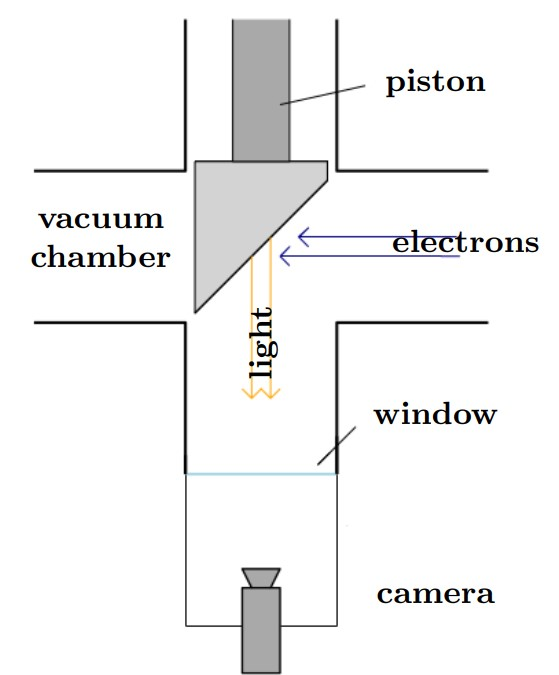
\includegraphics[width = 0.4\textwidth]{fig/screen.jpg}
    \caption{Schematic view of a used fluorescence screen \cite{lecturenote}.}
    \label{screen}
\end{figure}


\section{Measurement \& Analysis}
All steps of data analysis are done using Numpy library in Python \cite{numpy}. Linear and quadratic fitting is done with curve fit function of the Scipy model in Python \cite{scipy}. We solve all the equations when determining the emittance using the Python module Sympy \cite{sympy}.
\subsection{Verifying the Kick Angle Calibration}

We start by testing the calibration of the corrector magnets. While turning off quadrupoles, the kick angle of corrector magnets is alternated to measure the change in the associated beam position. For this, Corrector magnets C0 and C1 with their corresponding screens S0 and S1 are used. Only two corrector magnets are used since the beam broadens with distance. A calibration is verified by plotting the relative changes in positions against the set kick angles and checking whether there is a linear relation. Following a small angle approximation, the position offset, can be expressed as:

\begin{equation}
    \Delta x = tan (\alpha_x) L \simeq \alpha L 
    \label{eq5}
\end{equation}

\begin{equation}
    \Delta z = tan (\alpha_z) L \simeq \alpha L
    \label{eq6}
\end{equation}
Where $L$ represents the distance between the corrector magnet and its corresponding screen. Therefore, a slope of the fitting line of the correlation describes a drift length $L$ between a corrector magnetic and its associated screen as:
\begin{equation*}
    \frac{\partial x}{x'} \simeq L \simeq \frac{\partial z}{z'}
\end{equation*}

We quantify the correlation between the relative change of position in both the $x$ and $z$ direction and the kick angle. Then, data fitting is done using the curve fit function in Python. We plot the correlation for both directions in Figure \ref{kick angle} and present the resulting fitting parameters and their corresponding errors in Table \ref{tab1}. We also quantify the goodness of the fit by using the reduced chi-squared test and present the corresponding values in the labels of Figure \ref{kick angle} (The fit provides a good description of the data following the test of the goodness of the fit and shows that the relation is linear). 
\begin{table}[H]
    \centering
    \begin{tabular}{c|c|c|c}
    \hline
    \hline
         Screen & $\frac{\partial x}{\partial x'}$ $\mathrm{[m]}$ & $\frac{\partial z}{\partial z'}$ $\mathrm{[m]}$ & L $\mathrm{[m]}$ \\ 
    \hline
        $S_{0}$ & $0.267 \pm 0.002$ & $0.276 \pm 0.001$ & $0.24425$ \\ 
        $S_{1}$ & $0.482 \pm 0.005$ & $0.53 \pm 0.03$ & $0.37525$ \\ 
        \hline
    \end{tabular}
    
    \caption{Fitting parameters for the change in position against the kick angle of the corrector magnet.}
    \label{tab1}
\end{table}

When comparing the measured lengths described as slopes, with the actual lengths, presented in the last column of Table \ref{tab1}, we find that they are relatively in good agreement but not perfectly. This is due to the reason that the measured length is a measured effective length and not the actual distance and also, the applied kick is not given instantaneously.   


\begin{figure}[H]
    \centering
    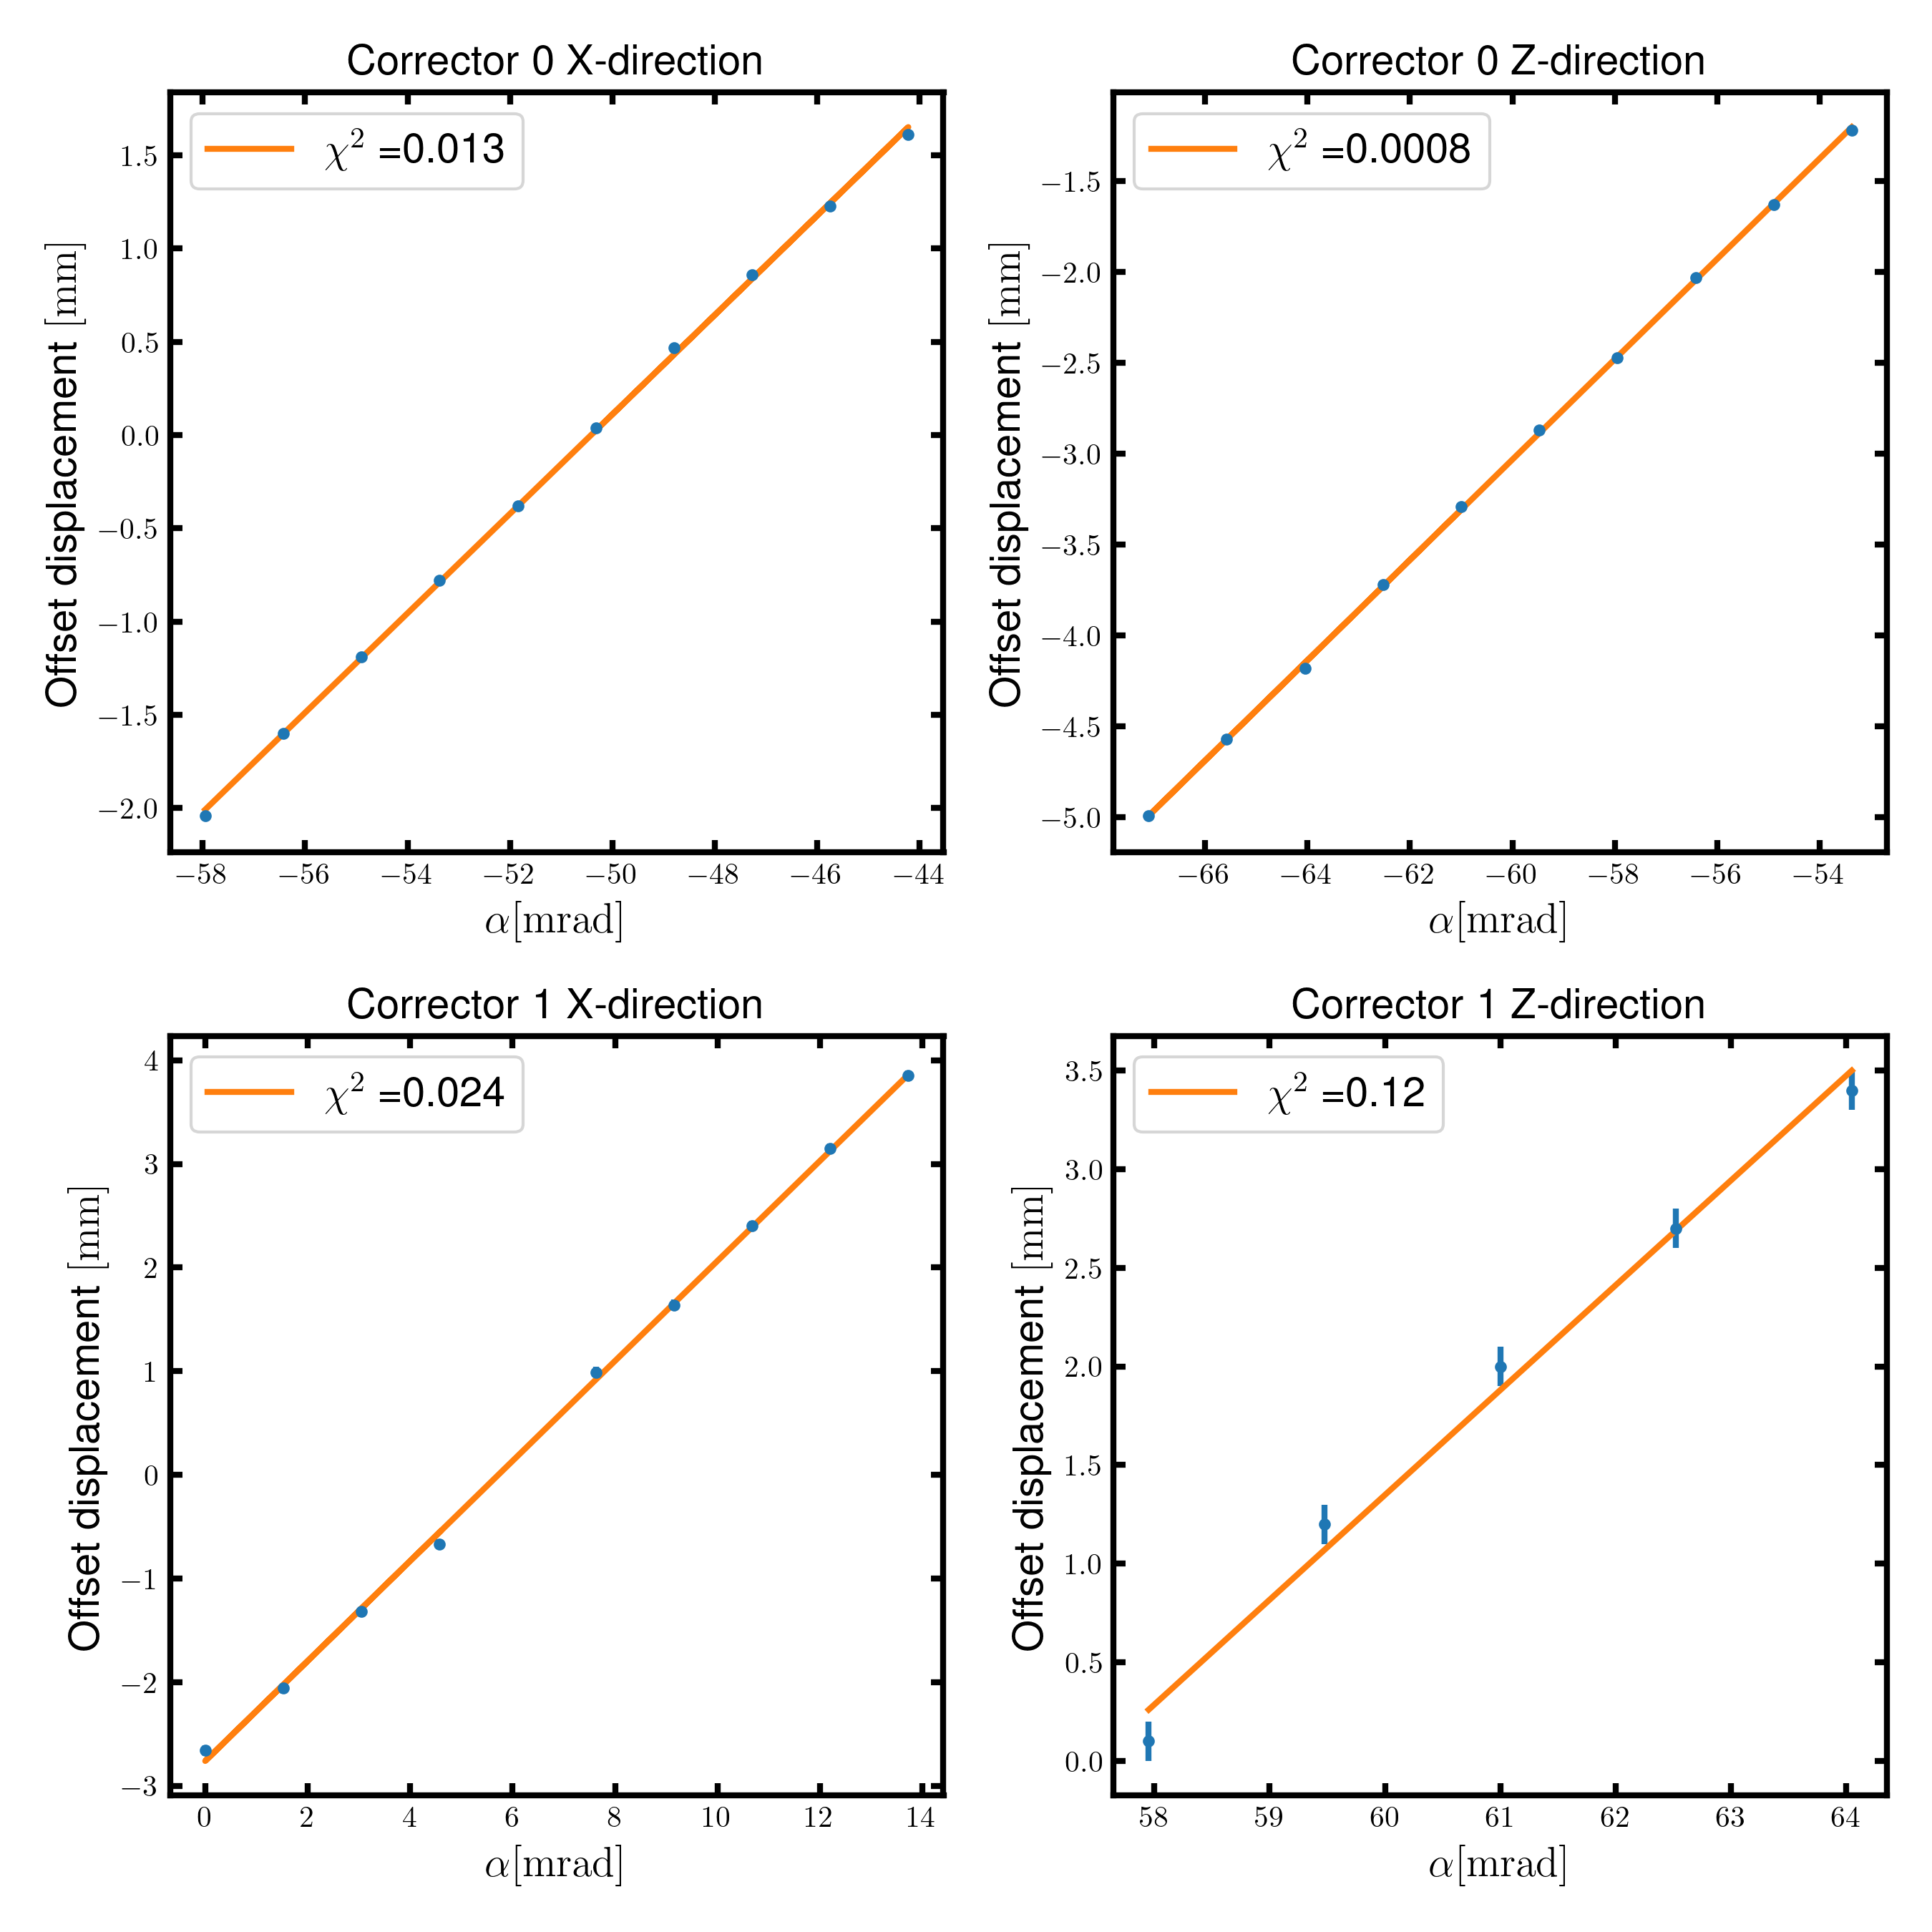
\includegraphics[width = 0.8\textwidth]{fig/displacement_by_angle_kickangle.png}
    \caption{Beam position in dependence of the applied kick angle in x and z direction. Error in the last subplot is higher as the peak position of the center of the beam was fluctuating relatively high in the z-direction.}
    \label{kick angle}
\end{figure}

Furthermore, we make a correlation plot between the 
angle set in the control system and the one calculated from equations \ref{eq5} and \ref{eq6} and show the results in Figure \ref{angle by angle}. 
Again, we do linear fitting similarly to the former case, show the goodness of the fit in the labels of Figure \ref{angle by angle}, and present the fitting parameters in Table \ref{tab2}. Slopes are close to one with slight deviations due to the same reasons mentioned in the previous case. Overall, one can say that the calibration is verified and optimization can be suggested for more improvements in the results. 

\begin{figure}[H]
    \centering
    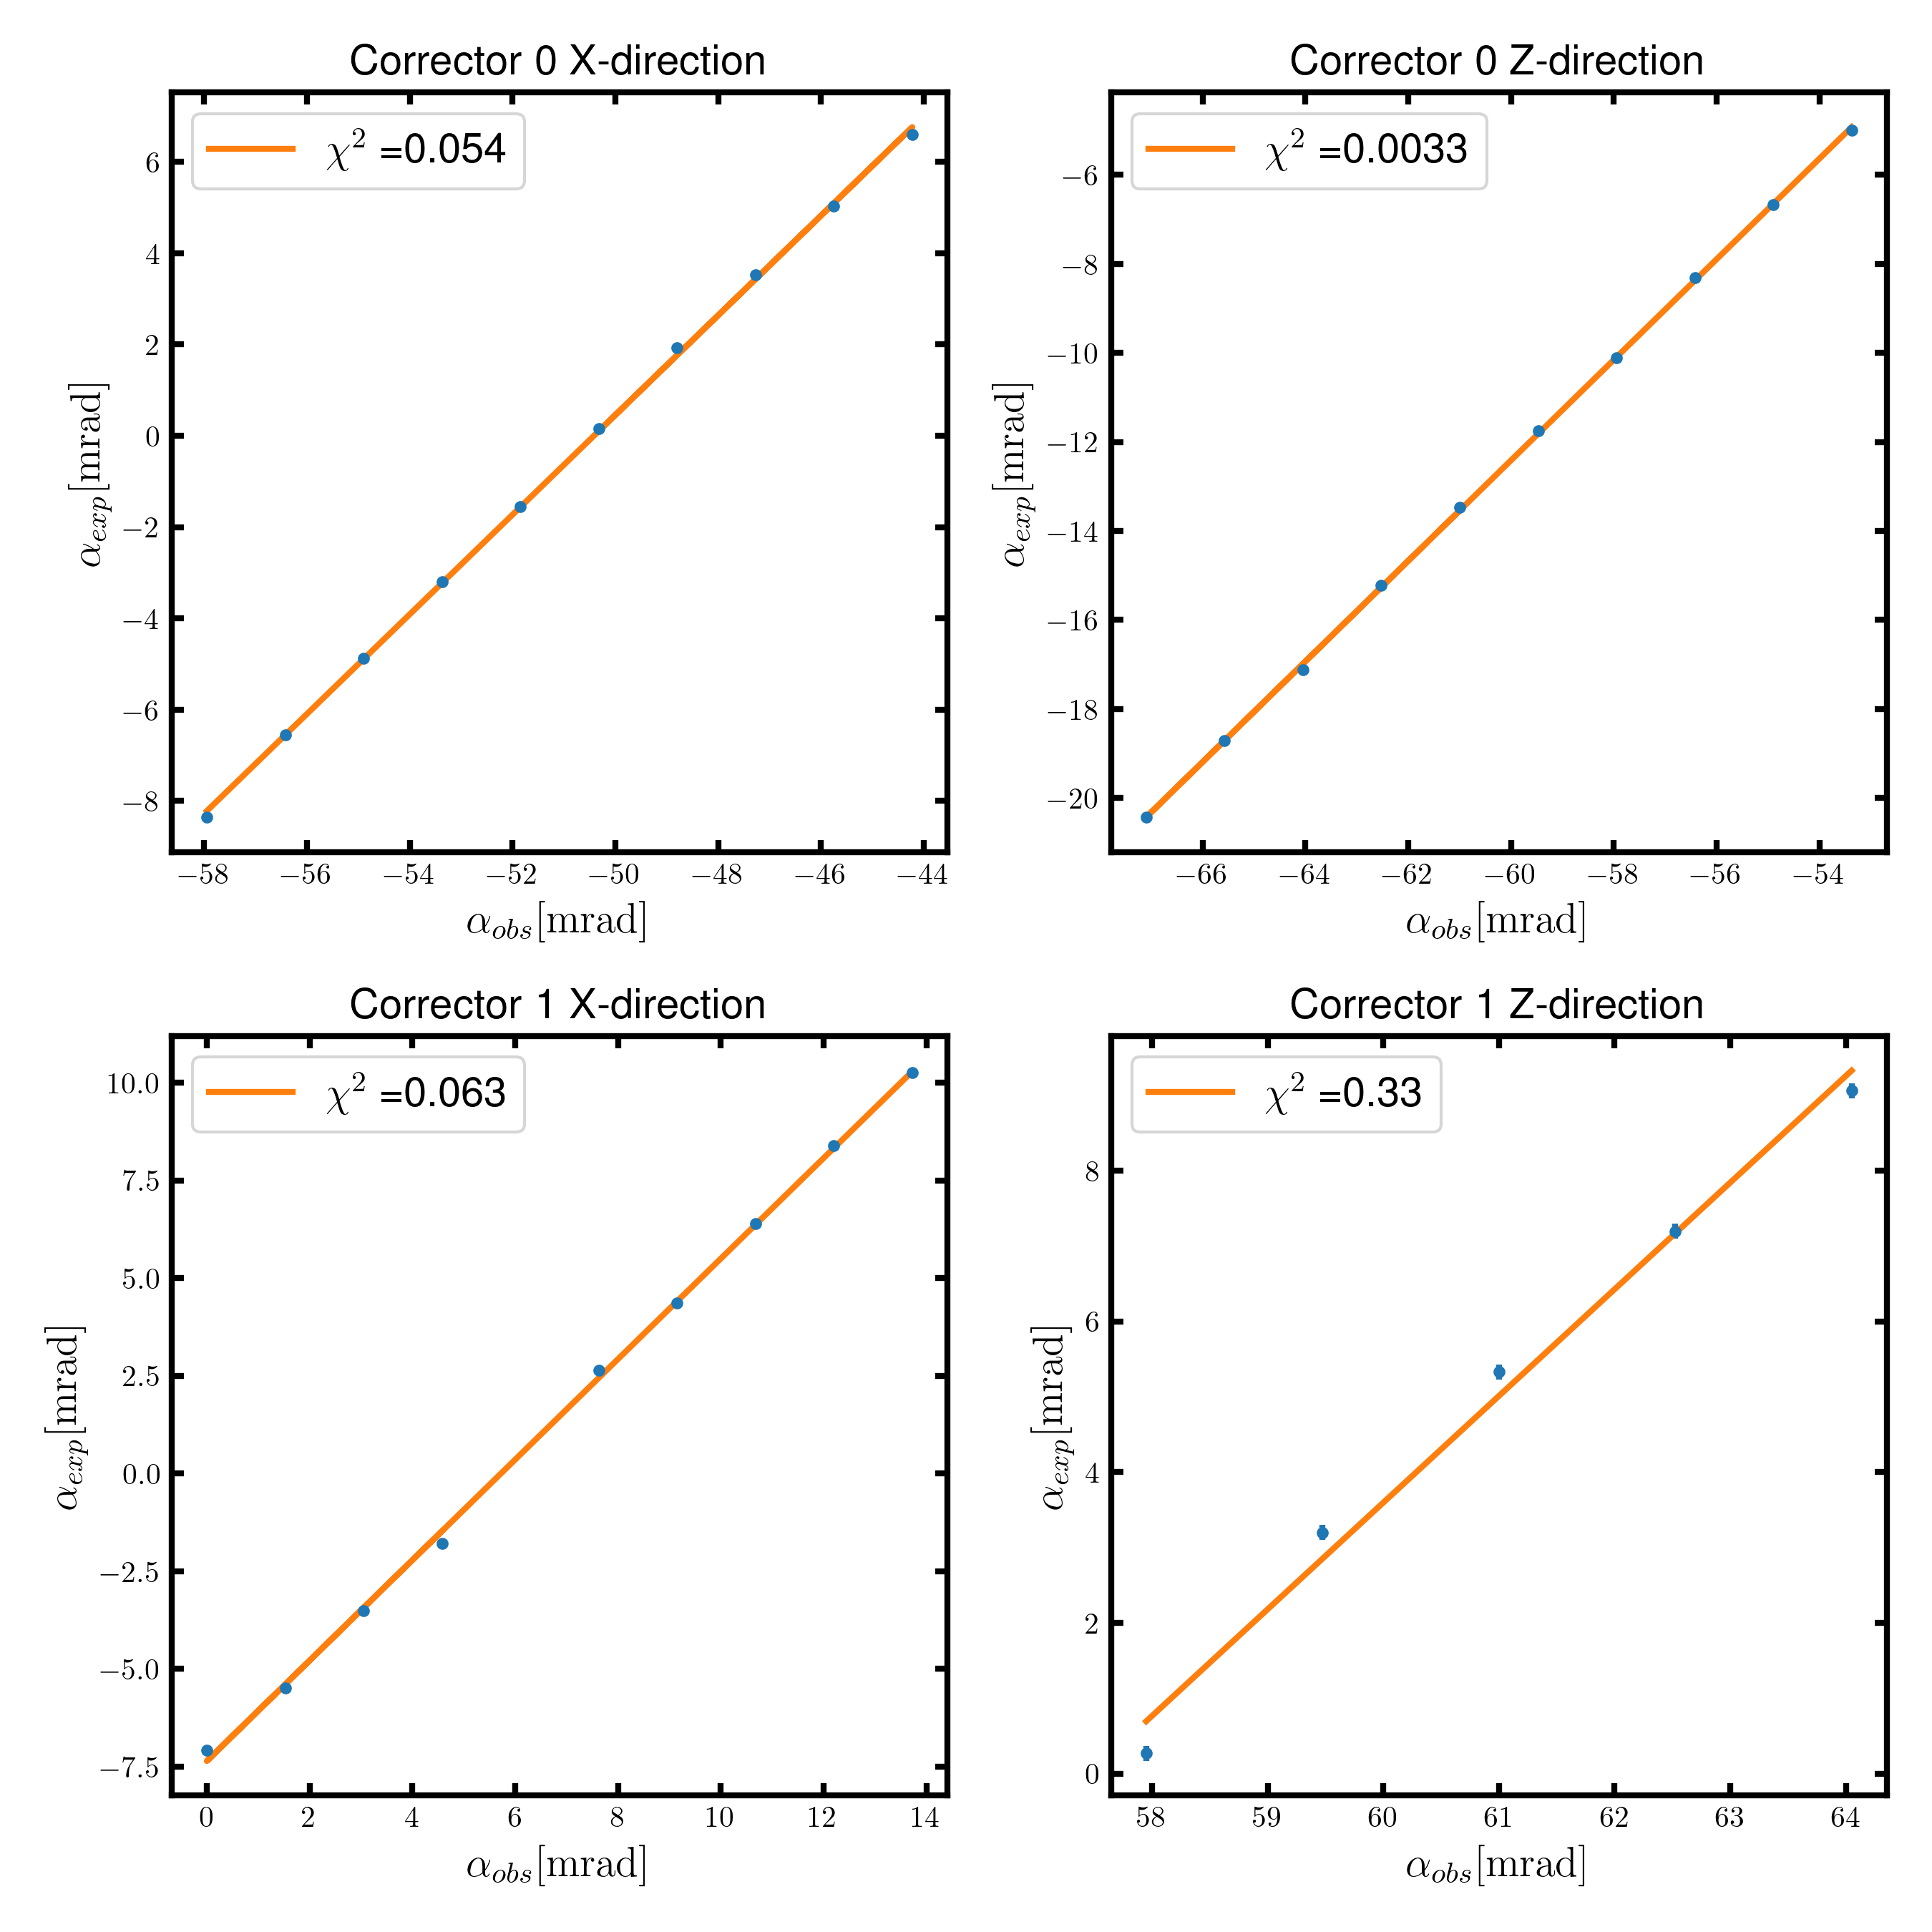
\includegraphics[width = 0.8\textwidth]{fig/angle_by_angle_kickangle.png}
    \caption{Kick angle set in the control system against the calculated on in both x and z direction.}
    \label{angle by angle}
\end{figure}


\begin{table}[H]
    \centering
    \begin{tabular}{c|c|c}
    \hline
    \hline
        Corrector & Slope X-direction  & Slope Z-direction \\ 
        \hline
        C0 & $1.091 \pm 0.008$ & $1.130 \pm 0.005$  \\ 
        C1 & $1.29 \pm 0.01$ & $1.42 \pm 0.08$ \\ 
    \hline
    
    \end{tabular}
    
    \caption{Fitting parameters of the correlation between the kink angle set in the control system against the calculated one in both x and z direction.}
    \label{tab2}
\end{table}

\subsection{Beam Based Alignment}

For every experiment done using a particle accelerator, alignment of the center of emitted beam is essential. This is to ensure that the beam passes through the quadrupole focusing magnets. In such a case, quadrupole magnets only focus the beam and no resulting magnetic kicks are realized.  

The procedure is as follows: The kick current of a corrector magnet in front of the quadrupole is used to set the position where the beam passes through the quadrupole. the strength of a quadrupole k is varied between two fixed values, spaced far apart enough, to allow significant deflection if the beam does not propagate through the center of a quadrupole. Following this, the resulting beam displacement $\Delta x$ and $\Delta z$ are measured on the screen behind the used quadrupole. 
The strength of the magnetic field of a quadrupole increases linearly outward and thus, the separation between $\Delta x$ and $\Delta z$ is proportional to the kick angle, kick current in our analysis. A condition of no deflection occurs for a separation of zero. This happens when the beam passes through the center of a quadrupole.  After each corrector magnet alignment, the corrector current in the control unit is fixed and not changed for the further corrector magnets. 

We plot the beam displacement in both the x and z direction for the first four corrector magnets against the applied kick current in Figure \ref{beam based alignment}. Then, a linear fitting is done and the goodness of the fit is analyzed and presented in Table \ref{tab3}, along with the ideal zero point values of the applied kick current.

\begin{figure}[H]
    \centering
    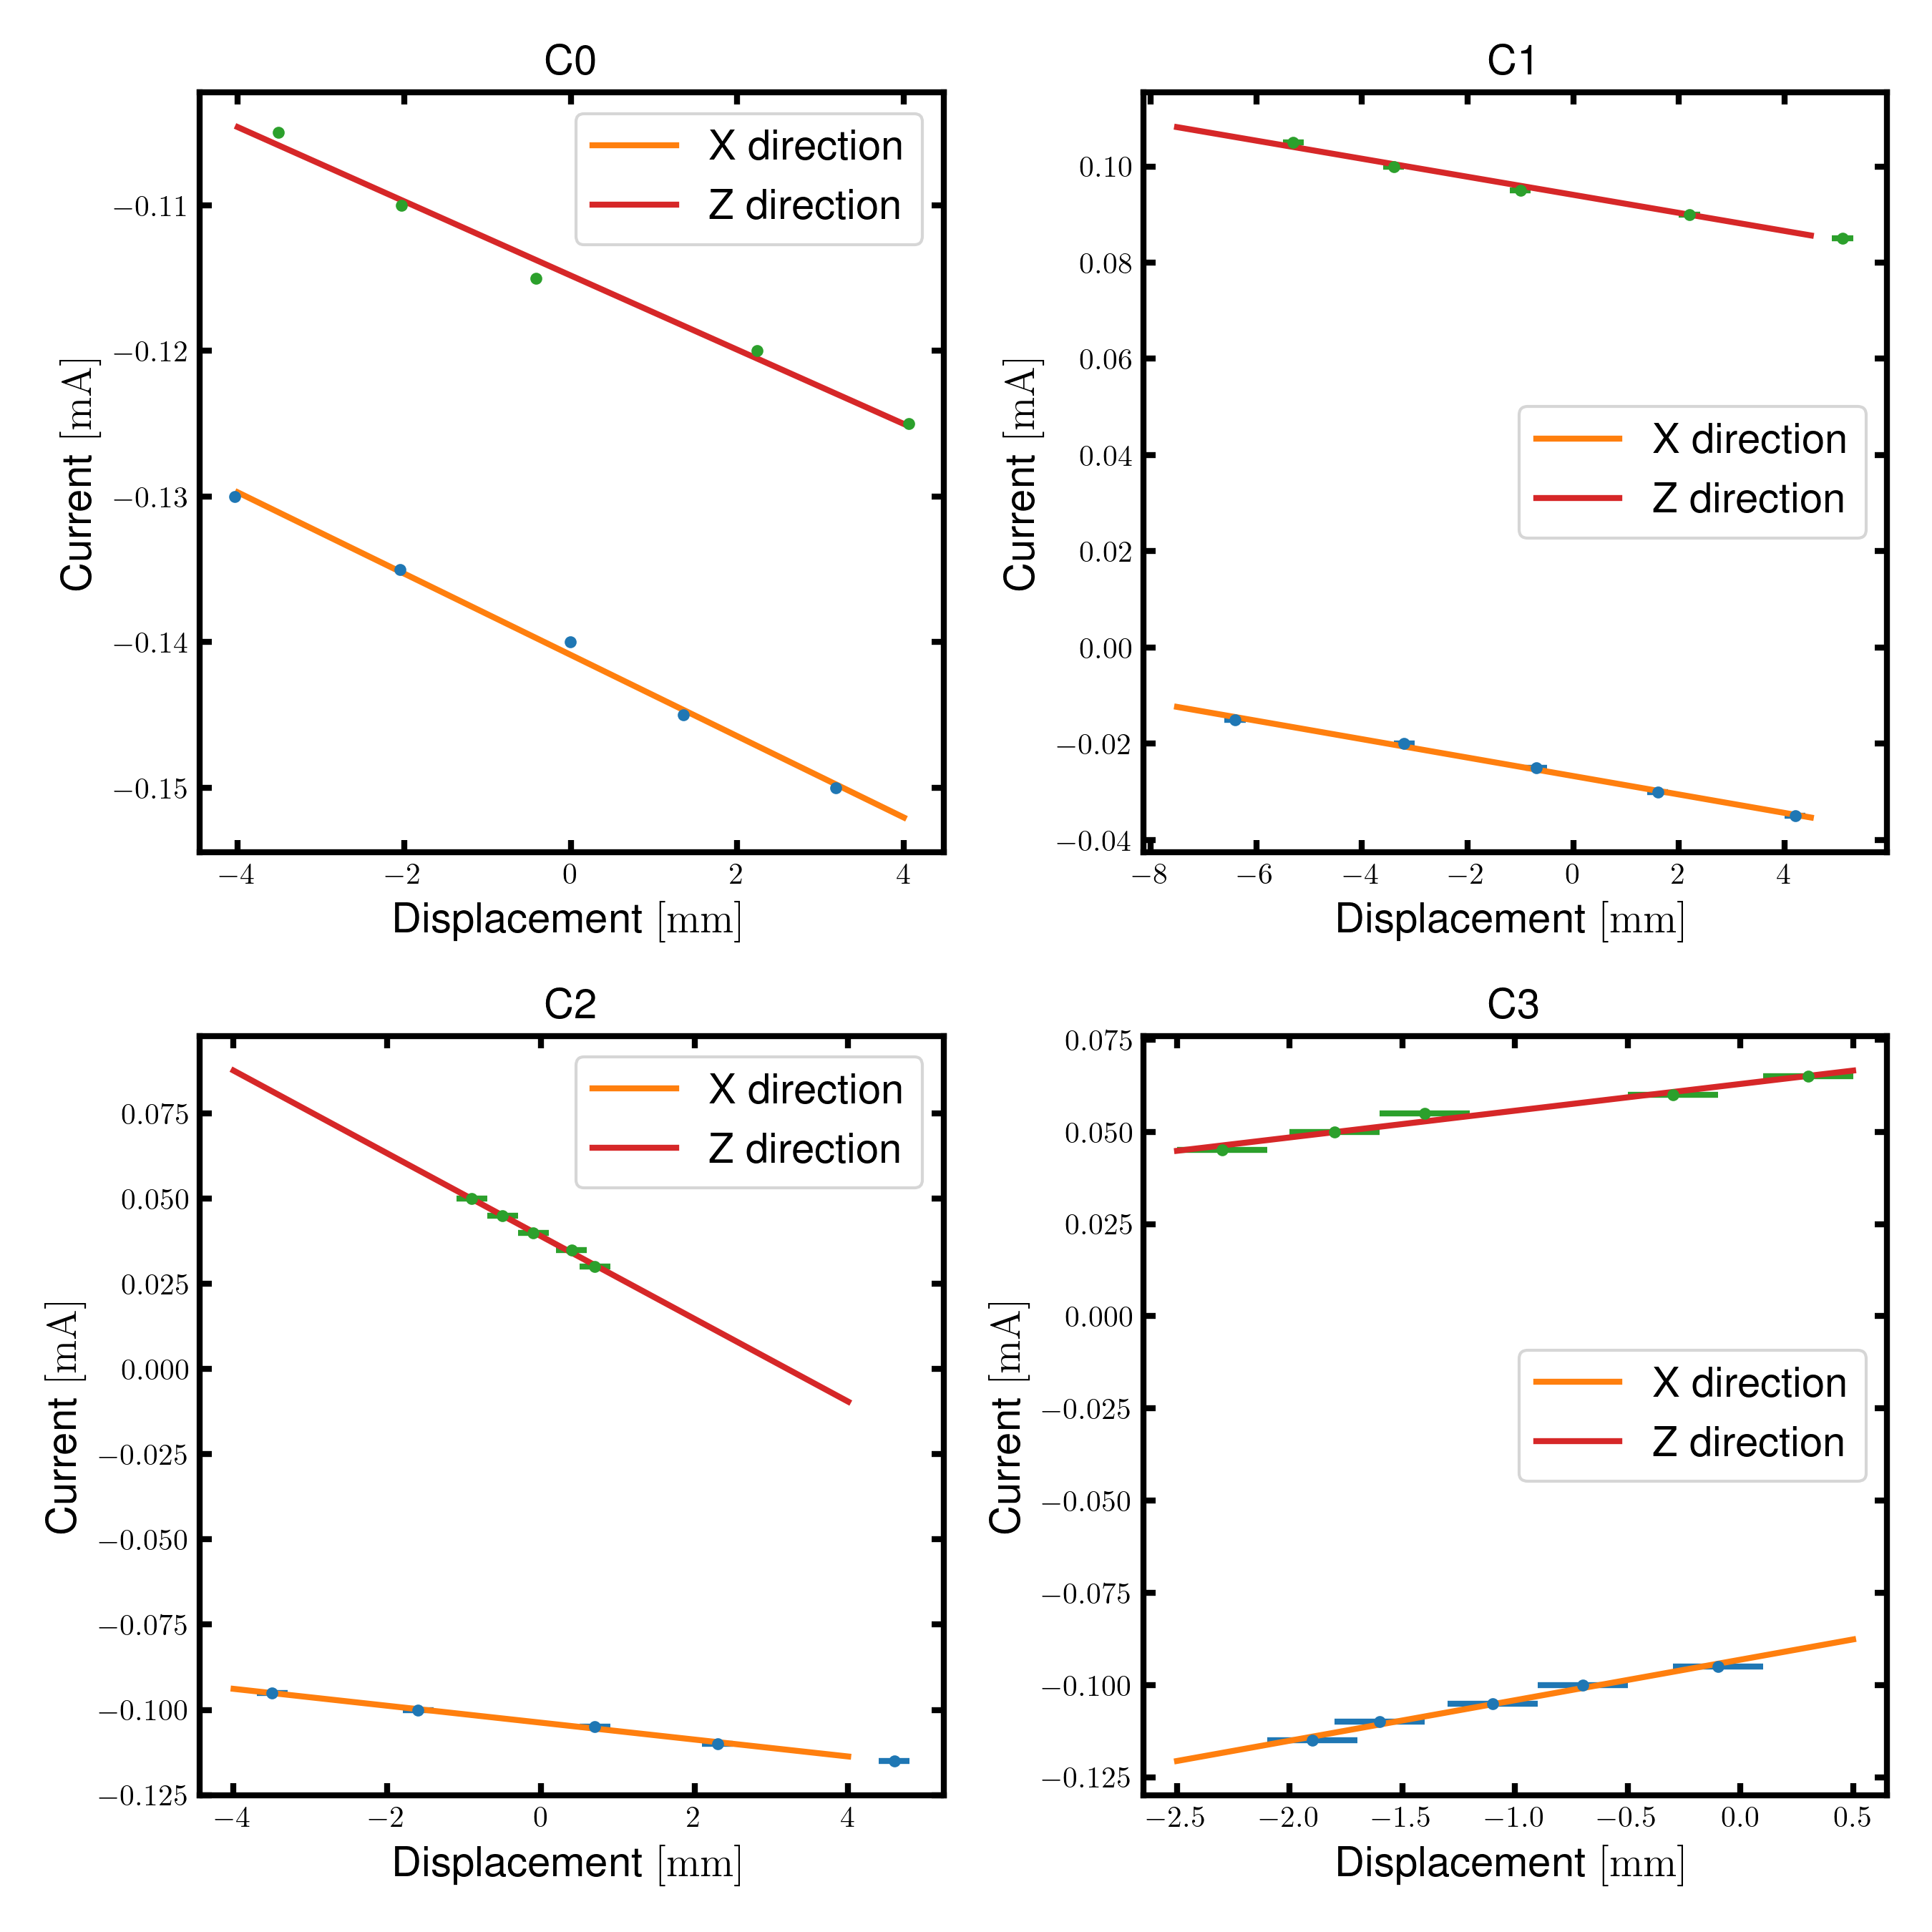
\includegraphics[width = 0.8\textwidth]{fig/beambasealinghment.png}
    \caption{Beam displacement in both the x and z direction for the first
four corrector magnets against the applied kick current.}
    \label{beam based alignment}
\end{figure}

\begin{table}[H]
    \centering
    \begin{tabular}{c|c|c|c|c}
    \hline
    \hline
       Corrector & $I^{x}_{ideal}$ $\mathrm{[mA]}$& $\chi^2_x$ & $I^{z}_{ideal}$  $\mathrm{[mA]}$& $\chi^2_y$ \\ 
    \hline
        C0 & $-0.140876 \pm 0.000272$ & $0.000056$ & $-0.114827 \pm 0.000429$ & $0.000221$ \\ 
        C1 & $-0.026725 \pm 0.000250$ & $0.002540$ & $0.094099 \pm 0.000396$ & $0.000242$ \\ 
        C2 & $-0.103759 \pm 0.000205$ & $0.000053$ & $0.039028 \pm 0.000265$ & $0.000930$ \\ 
        C3 & $-0.093135 \pm 0.000849$ & $0.000255$ & $0.062976 \pm 0.001045$ & $0.002664$ \\ 
    \hline
    
    \end{tabular}
    \caption{Ideal corrector currents for the first four corrector magnets obtained by beam based alignment.}
    \label{tab3}
\end{table}

\subsection{Beam Transport}
Now, we set the beam to be centered in the quadrupole such that the focusing is optimized. We set the quadrupoles alternately to focus and defocus to get the most focused beam on the last screen. We present the results of the beam profiles before the use of quadrupoles in Figure \ref{before quadrupole} and after the use of quadrupole in Figure \ref{after quadrupole}

\begin{figure}[H]
  \centering

 \begin{subfigure}{0.16\textwidth}
    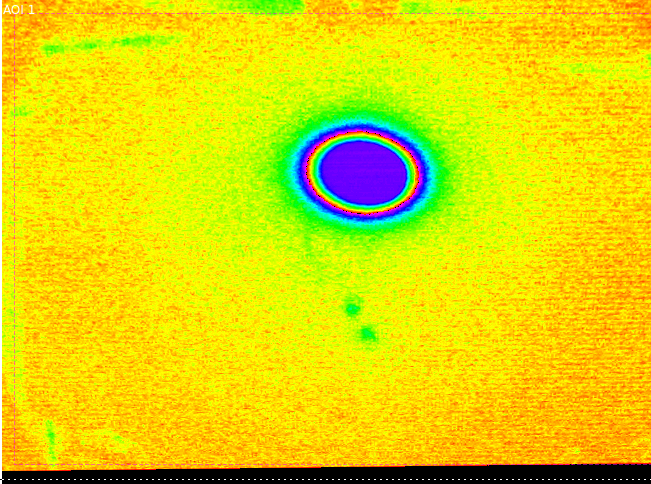
\includegraphics[width=\linewidth]{fig/S0w.png}
    \caption{$S_0$}
  \end{subfigure}%
  \hfill
  \begin{subfigure}{0.16\textwidth}
    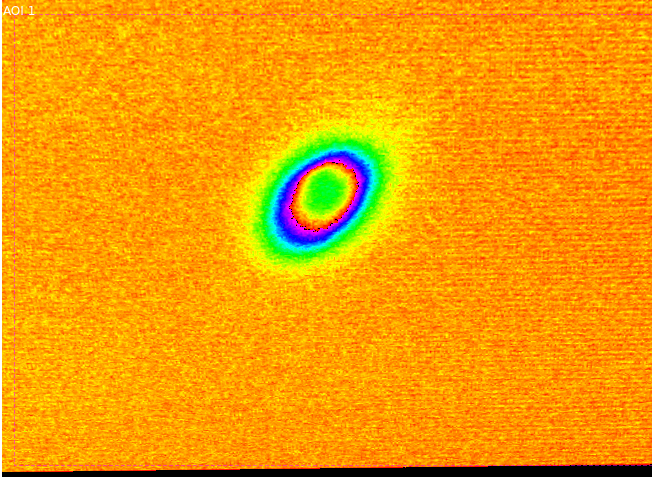
\includegraphics[width=\linewidth]{fig/S1.png}
    \caption{$S_1$}
  \end{subfigure}%
  \hfill
  \begin{subfigure}{0.16\textwidth}
    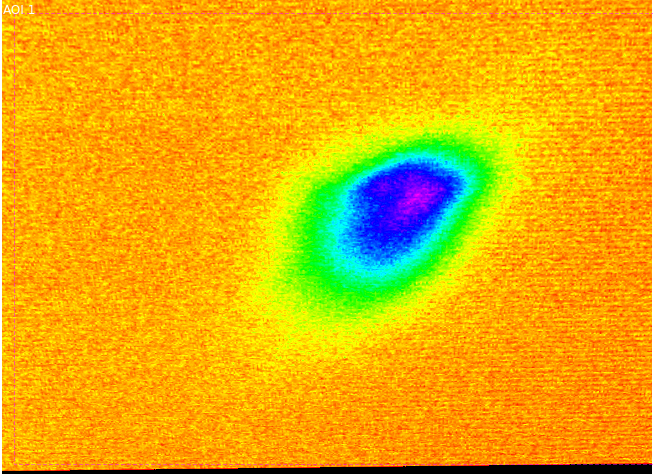
\includegraphics[width=\linewidth]{fig/S2.png}
    \caption{$S_2$}
  \end{subfigure}%
  \hfill
  \begin{subfigure}{0.16\textwidth}
    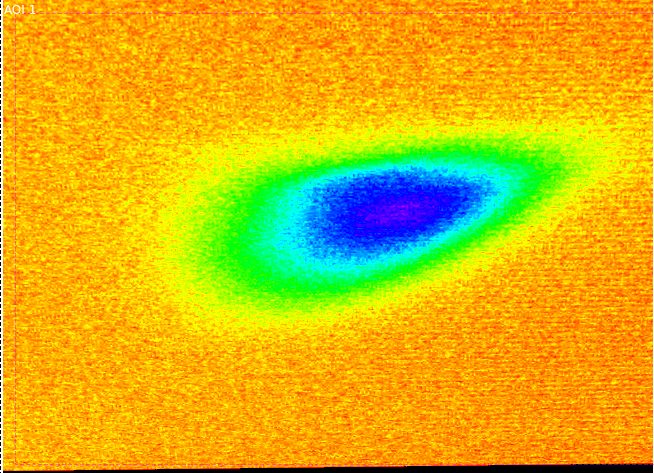
\includegraphics[width=\linewidth]{fig/S3.png}
    \caption{$S_3$}
  \end{subfigure}%
  \hfill
  \begin{subfigure}{0.16\textwidth}
    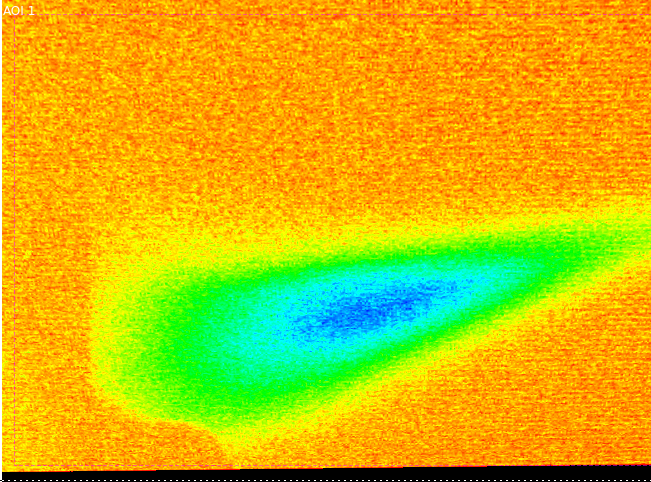
\includegraphics[width=\linewidth]{fig/S4.png}
    \caption{$S_4$}
  \end{subfigure}
 
  \caption{Screenshots of the beam profile at the screens $S_0$ to $S_4$ without the use of quadrupoles.}
  \label{before quadrupole}
\end{figure}





\begin{figure}[H]
  \centering

  \begin{subfigure}{0.16\textwidth}
    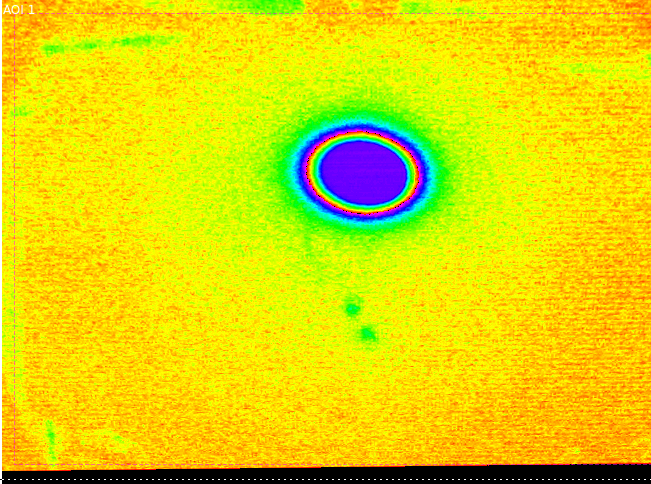
\includegraphics[width=\linewidth]{fig/S0w.png}
    \caption{$S_0$}
  \end{subfigure}%
  \hfill
  \begin{subfigure}{0.16\textwidth}
    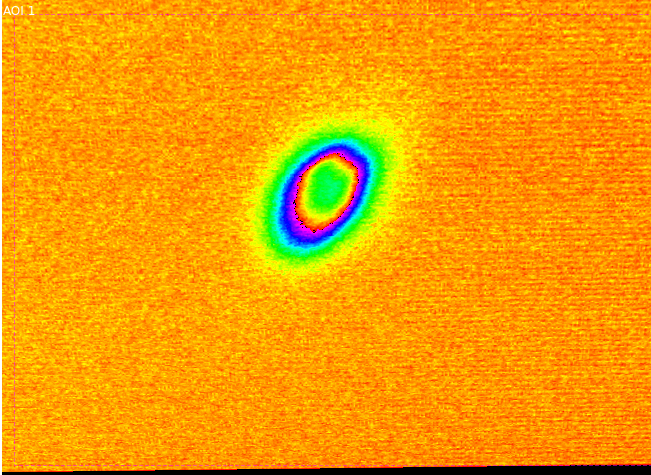
\includegraphics[width=\linewidth]{fig/S1w.png}
    \caption{$S_1$}
  \end{subfigure}%
  \hfill
  \begin{subfigure}{0.16\textwidth}
    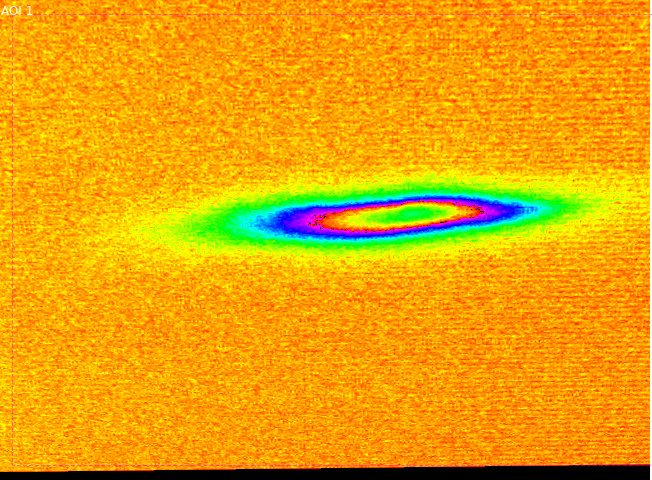
\includegraphics[width=\linewidth]{fig/S2w.png}
    \caption{$S_2$}
  \end{subfigure}%
  \hfill
  \begin{subfigure}{0.16\textwidth}
    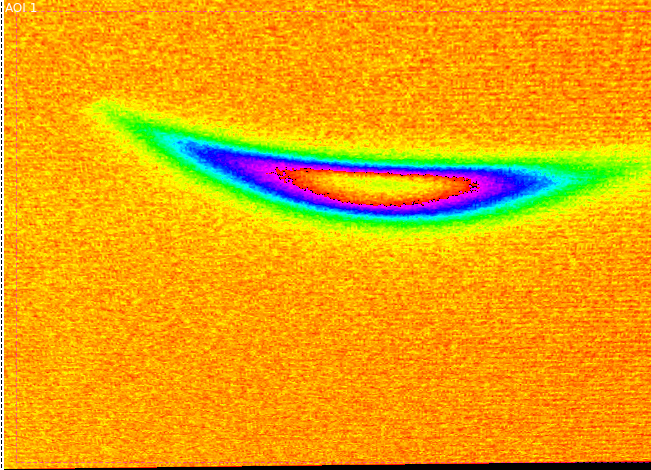
\includegraphics[width=\linewidth]{fig/S3w.png}
    \caption{$S_3$}
  \end{subfigure}%
  \hfill
  \begin{subfigure}{0.16\textwidth}
    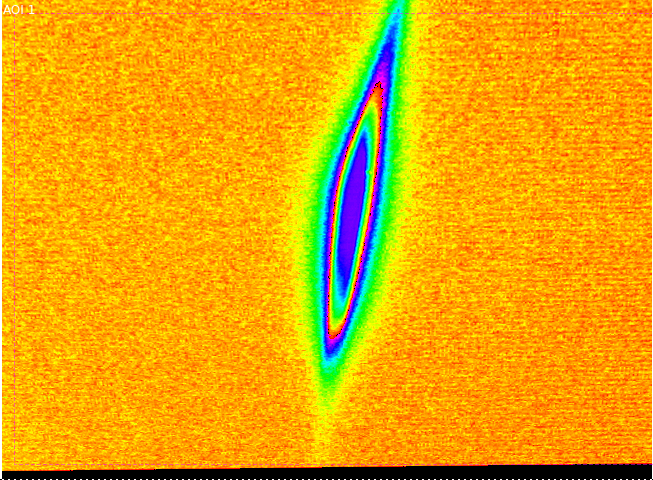
\includegraphics[width=\linewidth]{fig/S4w.png}
    \caption{$S_4$}
  \end{subfigure}
  
  \caption{Screenshots of the beam profile at the screens $S_0$ to $S_4$ after using quadrupole. Quadrupole strengths used [$1/m^2$]: 19.0, -42.7, 27.7, and 34.4, for the four quadrupoles respectively.}
  \label{after quadrupole}
\end{figure}

One can see from Figure \ref{before quadrupole}, that the beam increasingly losing focus, however, it gets focused after using the quadrupole, as shown in Figure \ref{after quadrupole}. 

\subsection{Beam Emittance Measurement}
A beam of electrons is all particle's individual trajectories combined. A beam envelope E(s) is described using the amplitude of a particle at 1 $\sigma$ of the overall  statistical distribution of single particle amplitudes and can be expressed as:

\begin{equation}
    E(s) = \sqrt{\epsilon \cdot \beta(s)}
\end{equation}

where $\epsilon$ is the beam emittance and $\beta(s)$ is the amplitude function. An example of a beam profile in one direction is depicted in Figure \ref{beam envelope}. The emittance provides a statistical quantification of the ability of an optical system to focus an emitted beam and $\beta(s)$ provides a description of the influence of the optical elements on the beam profile.

\begin{figure}[H]
    \centering
    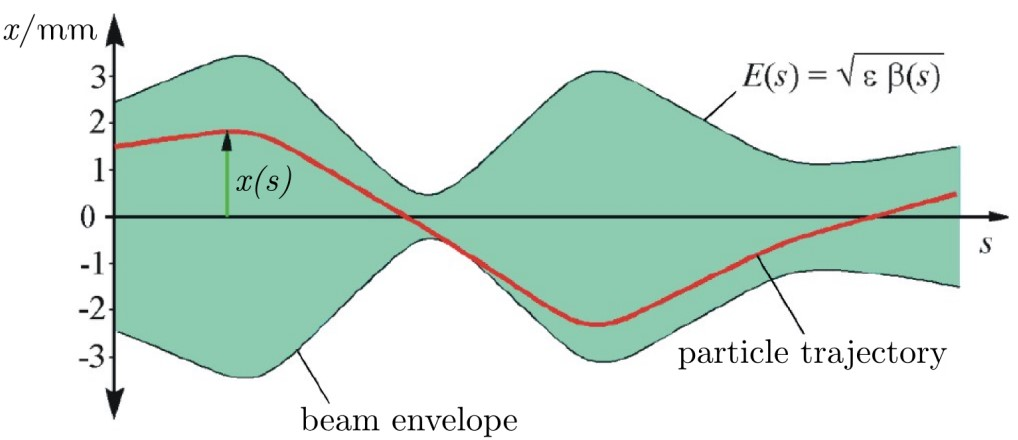
\includegraphics[width = 0.6\textwidth]{fig/beam envelope.jpg}
    \caption{An example of a beam envelope in x direction}
    \label{beam envelope}
\end{figure}

A visualization of the phase space, (x, x') or (z, z'), is shown in Figure \ref{phase space}. This phase space describes an ellipse with an area $F = \pi \epsilon$, which is a conserved quantity along the beam line. This ellipse can be described using parameters called Twiss parameters $\alpha (s)$, $ \beta (s)$, and $\gamma (s)$. Where $\beta (s)$ corresponds to the beam width ($\sigma_x$ or $\sigma_z$), $\gamma (s)$ corresponds to the angular width ($\sigma_{x^{'}}$ or $\sigma_{z^{'}}$), and $\alpha$ correlates both. Twiss parameters depend on the optics of the accelerator and thus, change along the beam line. To include the Twiss parameters in a matrix formalism, we use the Beta matrix, expressed as:
\begin{equation}
B (s) = 
    \begin{pmatrix}
    \beta (s) & -\alpha (s)  \\
    -\alpha (s) & \gamma (s)  \\
    
\end{pmatrix}
\label{beta matrix}
\end{equation}

Which is transformed via:

\begin{equation}
 B (s_1) = M \cdot B(s) \cdot M^T 
 \label{eq9}
\end{equation}
These two expressions are both valid for both x and z. When propagated along the beamline, the ellipse equation then reads:

\begin{equation}
\epsilon=(\vec{x}(s))^{\mathrm{T}} \cdot B_x(s)^{-1} \cdot \vec{x}(s)
\label{eq10}
\end{equation}

This relation \ref{eq10} will be used to determine the emittance using two methods: Quadrupole scan muthod and multi screens method. 



\begin{figure}[H]
    \centering
    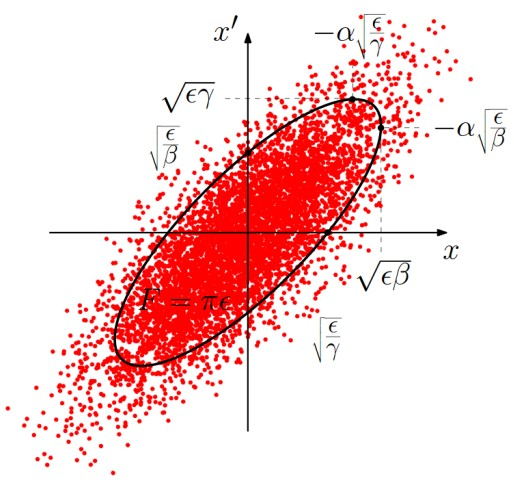
\includegraphics[width = 0.4\textwidth]{fig/phase space.jpg}
    \caption{Phase space ellipse in one place}
    \label{phase space}
\end{figure}

\subsubsection{Quardupole Scan Method}
The quadrupole scan is done twice for different locations. We use screen S2 with Q2 first and then S3 with Q3. We determine the beam emittance at both positions and expect similar values as the emittance is conserved along the beam line. 
If we rewrite eq. \ref{eq9} in terms of the beamwidth at a single screen position $s_1$, we get:
\begin{equation}
    \sigma_1^2(k)=m_{11}^2(k) \cdot\left(\epsilon \beta_0\right)-2 m_{11}(k) m_{12}(k) \cdot\left(\epsilon \alpha_0\right)+m_{12}^2(k) \cdot\left(\epsilon \gamma_0\right)
    \label{eq11}
\end{equation}

Where $m_{ij}$ represents the elements of the transfer matrix from a reference screen point $s_1$ to the location of the screen used for the measurement $s_2$.  When fitting eq. \ref{eq11}, to the measurement of $\sigma^{2}(k)$, one can obtain the parameters $(\epsilon \alpha),(\epsilon \beta)$ and $(\epsilon \gamma)$. 

The transfer matrix of the whole beamline is obtained by matrix multiplication of all optical elements in reverse order. A drift or a corrector element transfer matrix is expressed as:


\begin{equation}
M_x^{\mathrm{drift}}=M_z^{\mathrm{drift}}=\left(\begin{array}{ll}
1 & L \\
0 & 1
\end{array}\right)
\label{eq12}
\end{equation}

Where L is the length of an optical element. For quadrupole, the transfer element of an element, for a thin lens approximation, is expressed as:

\begin{equation}
M^{\mathrm{Q}}=\left(\begin{array}{cccc}
1 & L & 0 & 0 \\
-k L & 1 & 0 & 0 \\
0 & 0 & 1 & L \\
0 & 0 & k L & 1
\end{array}\right)
\label{eq13}
\end{equation}

Using the transfer matrices for drifts \ref{eq12} and quadrupoles \ref{eq13}, the transfer matrix to $S_2$ can be expressed as:

\begin{align}
    \begin{gathered}
        M^{\mathrm{Q} 2 \rightarrow \mathrm{S} 2}=M^{\mathrm{drift}} M^{\mathrm{C} 2} M^{\mathrm{drift}} M^{\mathrm{QF} 1} = \\
         \left(\begin{array}{cc}
        1.0 - 0.0328|k| & 0.5185 \\
        -0.074|k| & 1.0
    \end{array}\right) 
    \end{gathered}
    \label{eq14}
\end{align}

The C1 matrix represents a drift for the actual length of the corrector, where the final drift accounts for half of the screen's length and the distance between the corrector the screen. Drift values are taken from \cite{lecturenote} and absolute values $|k|$ are used since only one quadrupole is involved. The elements of \ref{eq14} are linear in k, thus, eq. \ref{eq11} represents a quadratic equation for $\sigma^{2}(k)$, expressed as:

\begin{equation}
\sigma^2(k)=a k^2+b k+c
\label{quadratic fit}
\end{equation}

We measure the beam width $\sigma$ in both directions and plot them in dependence on the applied quadrupole strength k for screen 2 and 3 in Figure \ref{quadrupole 2} and Figure \ref{quadrupole 3} respectively. 

\begin{figure}[H]
    \centering
    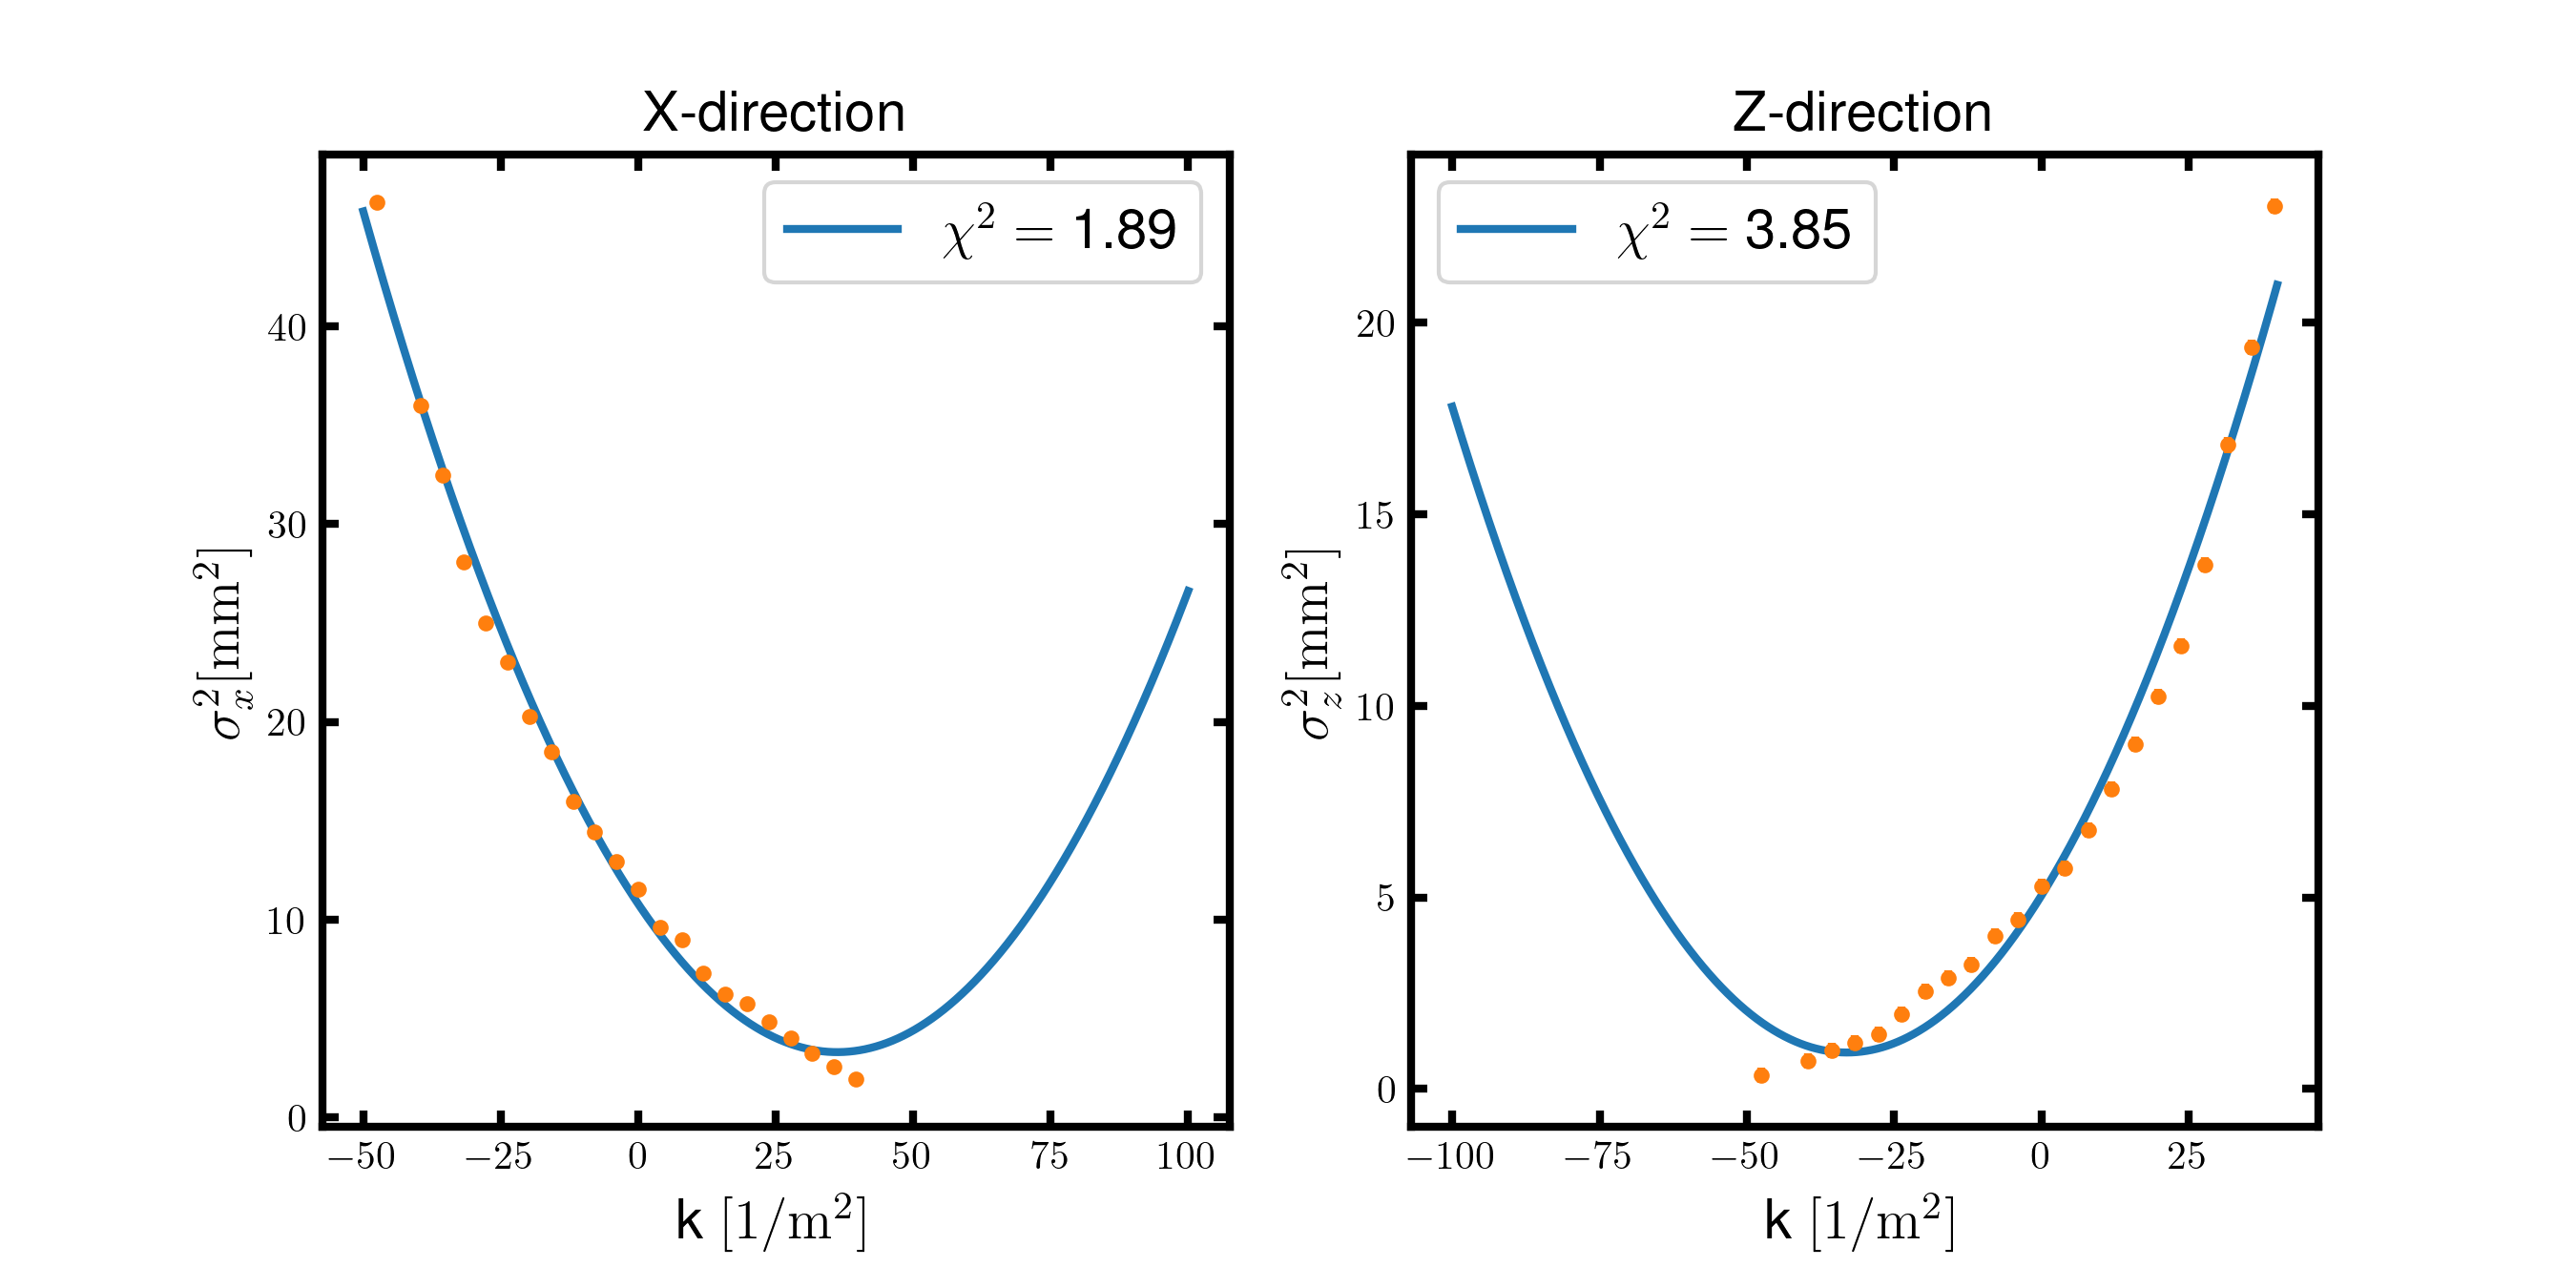
\includegraphics[width = \textwidth]{fig/Quadrupole_2.png}
    \caption{Beam width $\sigma^2$ in dependence of the applied quadrupole strength scanned on screen 2.}
    \label{quadrupole 2}
\end{figure}

\begin{figure}[H]
    \centering
    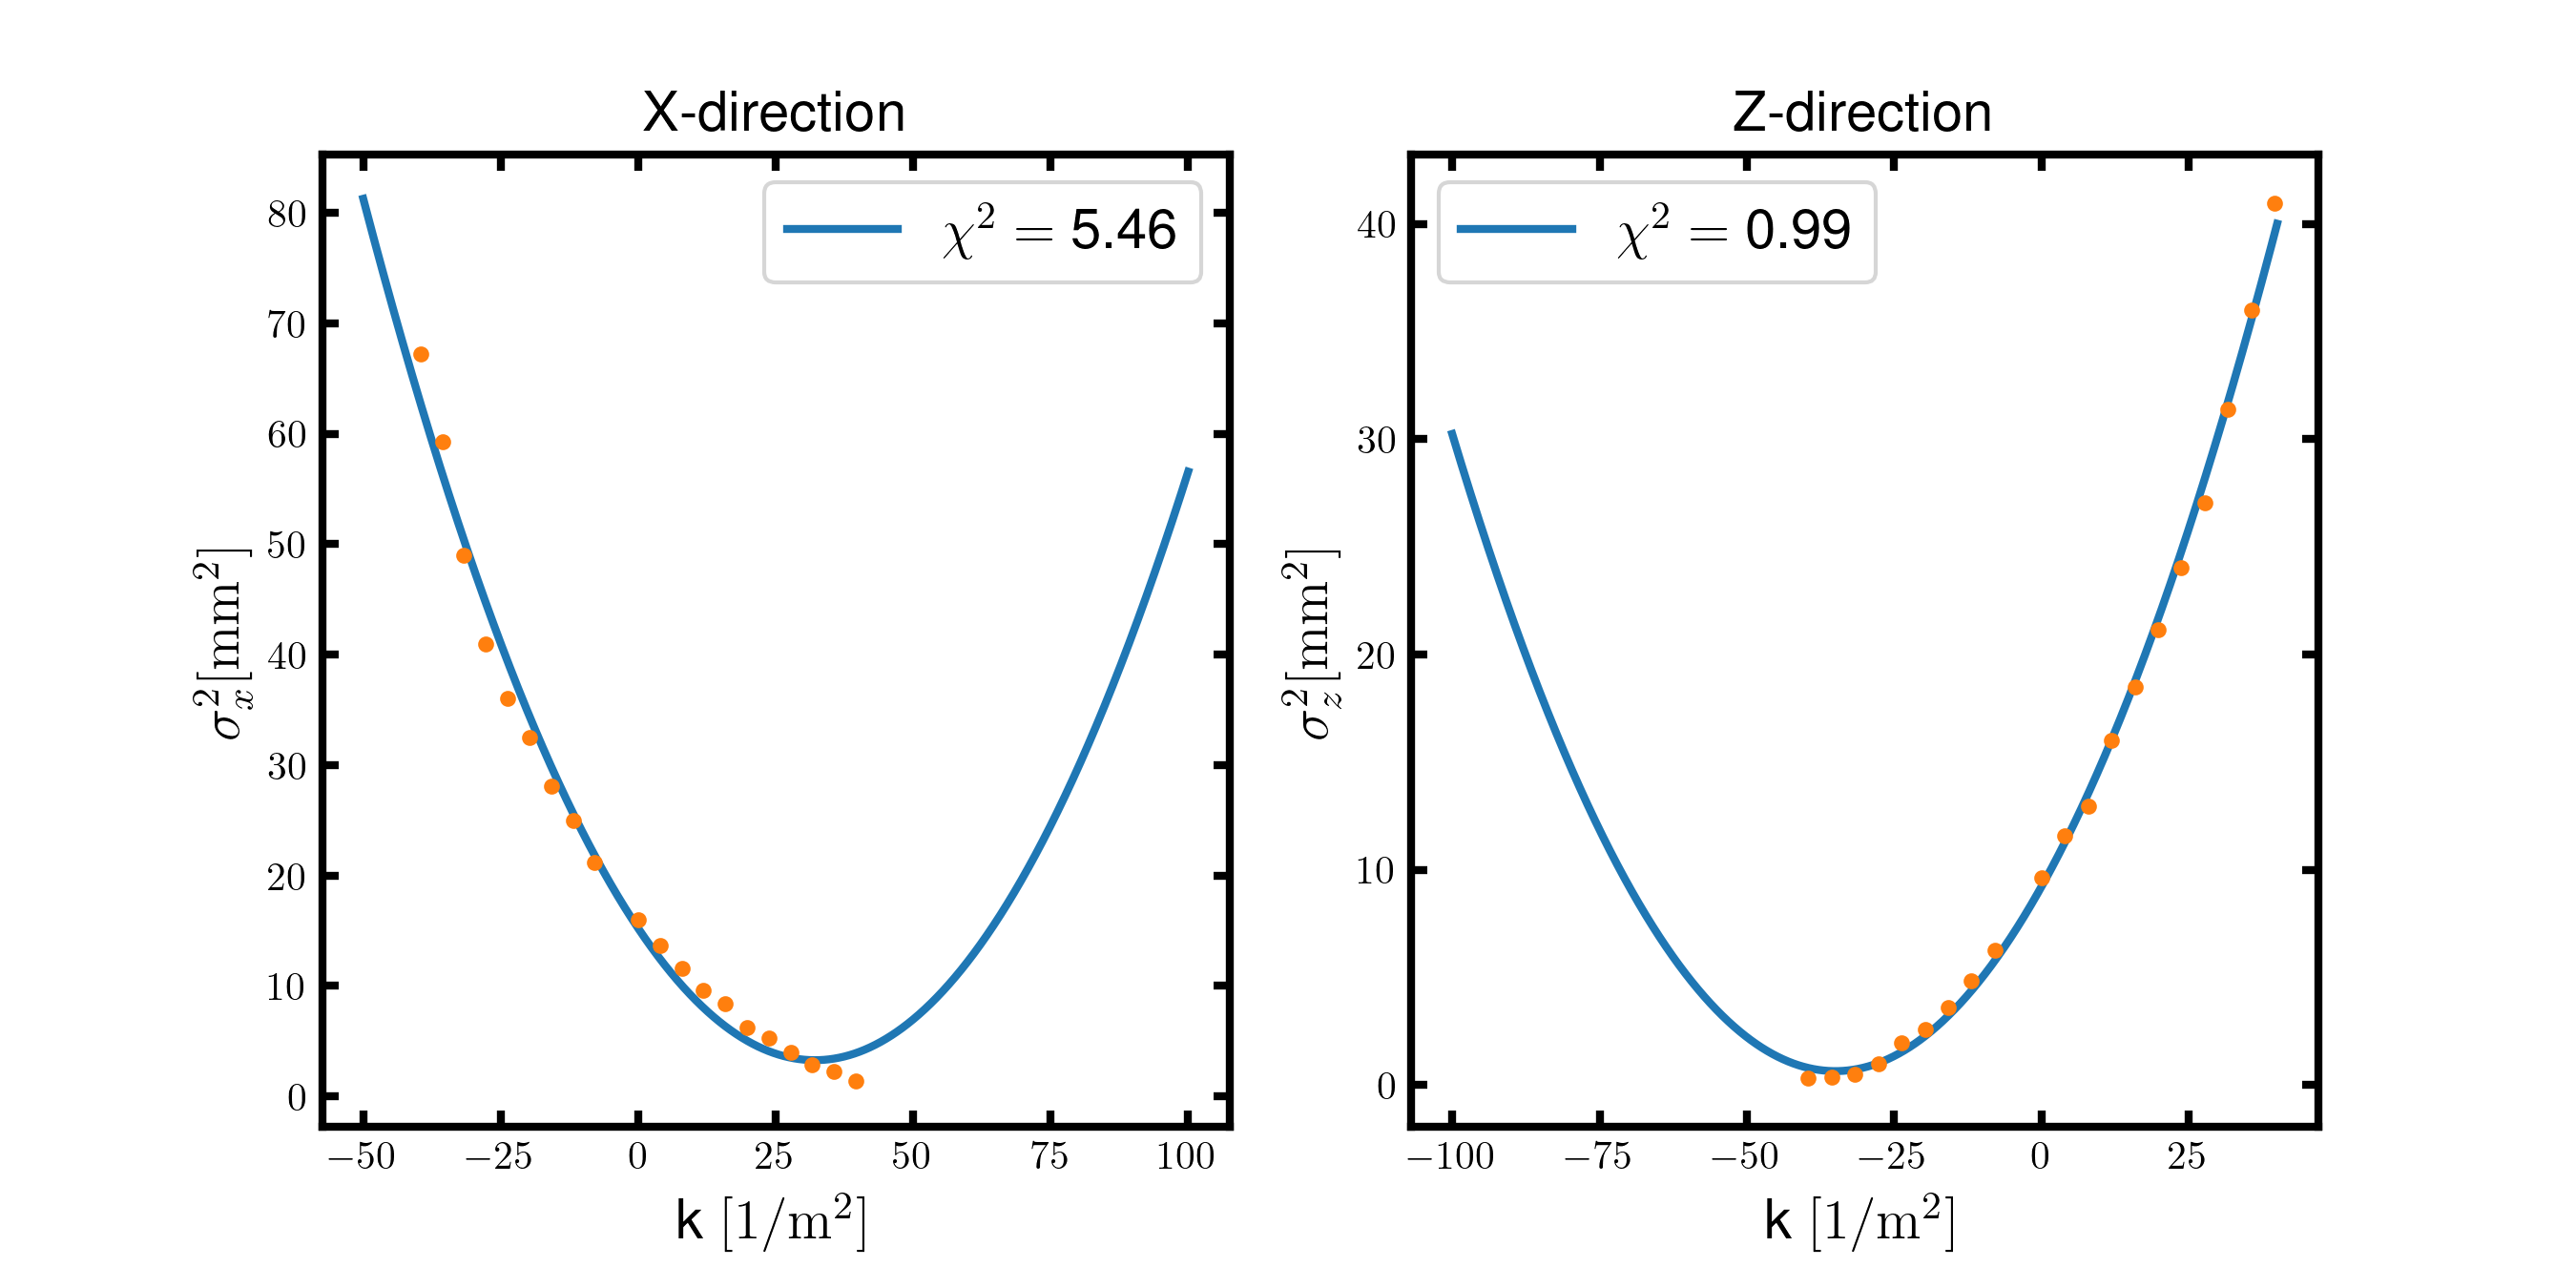
\includegraphics[width = \textwidth]{fig/Quadrupole_3.png}
    \caption{Beam width $\sigma^2$ in dependence of the applied quadrupole strength scanned on screen 3.}
    \label{quadrupole 3}
\end{figure}

We do a quadratic fit of the data and present the fitting parameters in Table \ref{quadratic_fit_table}. Furthermore, by equating the obtained fit function \ref{quadratic fit} with eq. \ref{eq11}, that corresponds to $S_2$, and solving the equation using Sympy library in Python \cite{sympy}, we obtain the Twiss parameters multiplied by the emittance, presented in Table \ref{Twiss parameters}. 


\begin{table}[H]
    \centering
    \begin{tabular}{c|c|c|c|c}
    \hline
    \hline
        Screen & Direction & a $\mathrm{[mm^2m^{-4}]}$ &b $\mathrm{[mm^2m^{-2}]}$ & c $\mathrm{[mm^2]}$ \\
    \hline
        S2& x & $0.0057 \pm 0.0004$ & $-0.414 \pm 0.009$ & $10.8 \pm 0.3$ \\ 
        S2& z & $0.0038 \pm 0.0003$ & $0.248 \pm 0.008$ & $5.1 \pm 0.3$ \\ 
        S3& x & $0.012 \pm 0.001$ & $-0.74 \pm 0.02$ & $15.2 \pm 0.8$ \\ 
        S3& z & $0.0070 \pm 0.0003$ & $0.490 \pm 0.006$ & $9.2 \pm 0.2$ \\
    \hline
    \end{tabular}
    \caption{Parameters of the quadratic fit applied on the data of quadrupole scans.}
    \label{quadratic_fit_table}
\end{table} 


% %%%%%%%%%%%%%%%%%%%%%%%%%%%%%%%%%%%%%%|||||S2|||||%%%%%%%%%%%%%%%%%%%%%%%%%%%%%


\begin{table}[H]
    \centering
    \begin{tabular}{c|c|c|c|c}
        \hline
        \hline
            Screen & Direction & $\epsilon \alpha_0$$\mathrm{[mm^2m^{-1}]}$ & $\epsilon \beta_0$$\mathrm{[mm^2]}$ &$\epsilon \gamma_0$$\mathrm{[mm^2m^{-2}]}$ \\ 
        \hline
            S2 & x & $10.592 \pm 4.479$ & $13.617 \pm 5.597$ & $13.022 \pm 3.652$ \\ 
            S2 & z & $2.916 \pm 1.691$ & $5.723 \pm 2.304$ & $3.633 \pm 1.371$ \\ 

        \hline
    \end{tabular}
    \caption{Twiss parameters multiplied by the beam emittance as obtained from the quadrupole scans.}
    \label{Twiss parameters}
\end{table}

A similar process is carried out for screen 3, employing a matrix identical to the one in \ref{eq14}, as the setup follows a repetitive pattern.


We present the fitting and Twiss parameters in Table \ref{tab6} and Table \ref{quadratic_fit_table}.

\begin{table}[H]
    \centering
    \begin{tabular}{c|c|c|c|c}
        \hline
        \hline
        Screen & Direction & $\epsilon \alpha_0$$\mathrm{[mm^2m^{-1}]}$ & $\epsilon \beta_0$$\mathrm{[mm^2]}$ &$\epsilon \gamma_0$$\mathrm{[mm^2m^{-2}]}$ \\ 
        \hline

        S3 & x & $18.122 \pm 15.795$ & $37.157 \pm 29.247$ & $12.357 \pm 8.608$ \\ 
        S3 & z & $2.719 \pm 1.991$ & $7.777 \pm 3.843$ & $2.949 \pm 1.075$ \\ 
        
        \hline
    \end{tabular}
    \caption{Parameters of the quadratic fit applied on the data of quadrupole
scans.}
    \label{tab6}
\end{table}

We were unable to achieve a perfect parabolic shape due to the challenge of focusing the beam to its minimum. As we attempted to reach this minimum focus point, we encountered difficulties as the beam was lost on the screen. Consequently, our data collection was limited to just before the point where the beam was lost. Specifically, for screens 2 and 3, we could not locate the minimum, except for the z-direction on screen 3. The primary cause of this error can be attributed to the double peak observed on the second screen. This double peak significantly affected the accuracy of measuring the relative distance, as the Gaussian fit peak changed due to this phenomenon. 


\subsubsection*{Emittance Via Determinant}

From the determinant of the Beta matrix \ref{beta matrix}, which is always equal to one, we get:

\begin{equation}
\epsilon^2=(\epsilon \beta) \cdot(\epsilon \gamma)-(\epsilon \alpha)^2
\label{emittance via determinant equation}
\end{equation}

We now use eq. \ref{emittance via determinant equation} with the parameters to determine the emittance while propagating the errors and present the results for screen 2 and 3 in Table \ref{tab:emittance via determinant}.

\begin{table}[H]
    \centering
    \begin{tabular}{c|c|c}
    \hline
    \hline
         Screen &   $\epsilon_x$ [$\mu$mrad] & $\epsilon_z $ [$\mu$mrad] \\
    \hline
         $S_2$ & $8.070 \pm 1.755$ &  $3.942 \pm 1.170$ \\
         $S_3$ & $11.434 \pm 5.314$ & $3.505 \pm 0.928$  \\
    \hline
    
    \end{tabular}
    \caption{Emittance via determinant for both directions.}
    \label{tab:emittance via determinant}
\end{table}
\subsubsection*{Emittance Via Measured Beam Waist}
By using eq. \ref{eq9} and setting $\alpha$ = 0, we obtain:

\begin{equation}
\epsilon^2=\sigma_w^2\left[m_{21}^2\left(s, k_w\right) \cdot\left(\epsilon \beta_0\right)-2 m_{21}\left(s, k_w\right) \cdot m_{22}\left(s, k_w\right) \cdot\left(\epsilon \alpha_0\right)+m_{22}^2\left(s, k_w\right) \cdot \gamma_0\right]
\label{eq18}
\end{equation}

A minimum of the of the quadratic fit function is considered to determine the properties of the beam waist. Therefore, a beam waist of a quadrupole strength is expressed as:
\begin{equation}
k_w=-\frac{b}{2 a}
\end{equation}

By reinserting this value into the fit function, we get the square of the beam waist width $\sigma^2_w$. Then, we calculate the transfer matrices similar to the case of using the determinant, but with inserting $k_w$. This makes the right hand side of eq. \ref{eq18} fully determined and allows for the calculation of the beam emittance. We present the results of the beam emittance and beam waist parameters in Table \ref{tab8} and Table \ref{tab9}. 
% #determminant 

\begin{table}[H]
    \centering
    \begin{tabular}{c|c|c}
    \hline
    \hline
         Screen &  $\epsilon_x$ [$\mu$mrad] & $\epsilon_z $ [$\mu$mrad] \\
    \hline
         $S_2$ & $ 11.586 \pm 0.384$ & $5.087 \pm 0.569$  \\
         $S_3$ & $14.866 \pm 0.795$ & $6.016 \pm 0.540$  \\
    \hline
    
    \end{tabular}
    \caption{Emittance via measured beam waist for both directions.}
    \label{tab8}
\end{table}

\begin{table}[H]
    \centering
    \begin{tabular}{c|c|c}

         &  $S_2$ & $S_3$\\
    \hline
         $k_{w,x}$ $\mathrm{[m^{-2}]}$ & $ 36.169 \pm 2.586 $  & $ 32.114 \pm 2.883 $ \\
         $\sigma^2_{w,x}$ $\mathrm{[mm^{2}]}$ & $ 3.311 \pm 0.698 $
            & $ 3.288 \pm 1.441$\\
         
         $k_{w,z}$ $\mathrm{[m^{-2}]}$ & $ -33.029 \pm 3.225 $& $ -34.986 \pm 1.391 $\\
         
         $\sigma^2_{w,z}$ $\mathrm{[mm^{2}]}$& $ 0.9508 \pm 0.555 $ & $ 0.646 \pm 0.434$\\
    \hline
    \end{tabular}
    \caption{Beam Twiss parameters for both directions.}
    \label{tab9}
\end{table}



\subsubsection{Multi-Screen Method}


To calculate the emittance using the multi-screen method, we measure the beam width $\sigma$ at all four screens while keeping the quadrupole strengths constant. Then by using the equation \ref{eq9}, we find a sets of linear equations: 

%%%%%%%%%
\begin{equation}
\overbrace{\left(\begin{array}{c}
\sigma^2\left(s_1\right) \\
\sigma^2\left(s_2\right) \\
\sigma^2\left(s_3\right) \\
\sigma^2\left(s_4\right)
\end{array}\right)}^{\vec{\sigma}}=\overbrace{\left(\begin{array}{lll}
m_{11}^2\left(s_1\right) & -2 m_{11}\left(s_1\right) m_{12}\left(s_1\right) & m_{12}^2\left(s_1\right) \\
m_{11}^2\left(s_2\right) & -2 m_{11}\left(s_2\right) m_{12}\left(s_2\right) & m_{12}^2\left(s_2\right) \\
m_{11}^2\left(s_3\right) & -2 m_{11}\left(s_3\right) m_{12}\left(s_3\right) & m_{12}^2\left(s_3\right) \\
m_{11}^2\left(s_4\right) & -2 m_{11}\left(s_4\right) m_{12}\left(s_4\right) & m_{12}^2\left(s_4\right)
\end{array}\right)}^M \cdot \overbrace{\left(\begin{array}{c}
\epsilon \alpha_0 \\
\epsilon \beta_0 \\
\epsilon \gamma_0
\end{array}\right)}^{\vec{x}}
\label{eq20}
\end{equation}
%%%%%%%%%%

To achieve beam focal spots in both the horizontal and vertical directions, alternating quadrupole strengths have been employed. The transfer matrix elements are computed, following the procedure outlined in the previous part, for each screen. the result of these matrices is shown in \ref{TM}.
All matrix calculations and solving equations are done with Sympy package in Python.

\begin{equation}
\begin{array}{ll}

M_x\left(s_1\right)=\left(\begin{array}{cc}
0.375 & 0.739 \\
-1.405 & 0.173
\end{array}\right) & 

M_z\left(s_1\right)=\left(\begin{array}{cc}
1.625 & 1.475 \\
 1.405 & 1.827
\end{array}\right) \\


M_x\left(s_2\right)=\left(\begin{array}{ll}
 -0.096 & 1.902 \\
 -0.574 & 2.555
\end{array}\right) & 

M_z\left(s_2\right)=\left(\begin{array}{cc}
 0.024  & 0.289  \\
 -4.088 & -3.298
\end{array}\right) \\


M_x\left(s_3\right)=\left(\begin{array}{cc}
 -0.329  & 1.786 \\
 -0.324 & -1.145
\end{array}\right) & 

M_z\left(s_3\right)=\left(\begin{array}{cc}
 -2.659 & -1.664 \\
 -4.619 &  -3.252
\end{array}\right) \\


M_x\left(s_4\right)=\left(\begin{array}{cc}
 -0.126 & -0.796 \\
 0.569 & -5.412
\end{array}\right) &

M_z\left(s_4\right)=\left(\begin{array}{cc}
 -8.813 & -5.763 \\
 -12.245 & -8.096
\end{array}\right)
\end{array}
\label{TM}
\end{equation}

Twiss parameter obtained from solving equations \ref{eq20} are shown in Table \ref{Twiss multi} 


\begin{table}[H]
    \centering
    \begin{tabular}{c|c|c|c}
    \hline
    \hline
        Direction & $\epsilon \alpha_0$ $\mathrm{[mm^2m^{-1}]}$ & $\epsilon \beta_0$ $\mathrm{[mm^2]}$ &$\epsilon \gamma_0$ $\mathrm{[mm^2m^{-2}]}$ \\
         \hline
         $x$ & 14.009 & 40.411 & 7.372 \\
         $z$ & 7.140 & 9.940 & 5.552 \\
    \hline
    \end{tabular}
    \caption{Twiss parameter for multi-screen method}
    \label{Twiss multi}
\end{table}

 For measuring the emittance from twiss parameters, equation \ref{emittance via determinant equation} is used and results are presented in Table \ref{emittance multi}

\begin{table}[H]
    \centering
    \begin{tabular}{c|c}
    \hline
    \hline
          $\epsilon_x$ [$\mu$mrad] & $\epsilon_z $ [$\mu$mrad] \\
    \hline
          $10.08 \pm 0.24$ &  $2.049 \pm 0.043$ \\
    \hline
    
    \end{tabular}
    \caption{Emittance in multi-screen method for both directions.}
    \label{emittance multi}
\end{table}


\section{Discussion}

In the kick angle verification section, we observed a 9\% deviation in the first screen from the expected value in the $x$ direction and a 13\% deviation in the $z$ direction. However, for the second screen, this deviation increased dramatically to approximately 30\% in the $x$ direction and 40\% in the $z$ direction. We can say that we successfully verified the kick angle for the first corrector. However, for the second corrector, it is not feasible to verify the kick angle due to substantial deviations from the expected value.

The primary cause of this error can be attributed to the double peak observed on the second screen. This double peak significantly affected the accuracy of measuring the relative distance, as the Gaussian fit peak changed due to this phenomenon, this is only done for the multiscreen method. 

In the quadrupole scan section, we encountered difficulties in obtaining a perfect parabolic curve. Instead, we were only able to obtain half of the parabolic shape, as evidenced in Figures \ref{quadrupole 2} and \ref{quadrupole 3}. Given the challenges in acquiring accurate data, it is not surprising that a significant error might be present in our results.

The source of the error appears to be a problem with the electron gun and the two solenoids following it, the current of the solenoids was changed making the resulting magnetic field used to focus the beeam different.  This issue prevented us from achieving a properly focused beam from the electron gun.

For error calculation, The errors were estimated by inserting the lower and upper values of the fit parameters into the equation system, and then re-solving for the Twiss parameters and emittance. 

\section{Conclusion}
A verification of the calibration of the system was done and the results showed that it was correct, despite some deviations due to errors discussed in the discussion part. Then, the beam is aligned to ensure that the beam passes through
the quadrupole focusing magnets. Furthermore, the beam emittance was measured using two methods: Quadrupole scan and Multi-screen. In the first one, the measurement is done at fixed positions with varying quadrupole strength k and we obtained the values in two ways, from the determinant of the Beta matrix and from the beam waist. In the second method, measurement is done at varying positions at a fixed $k$.
The obtained results are shown in Table \ref{final table}. 


\begin{table}[H]
    \centering
    \begin{tabular}{cccc}
        \hline 
        \hline
        Method & & $\epsilon_x$ [$\mu$mrad] & $\epsilon_z$ [$\mu$mrad] \\
        
        \hline \multirow{3}{*}{ Quadrupole Scan } & Determinant at $S_2$ & $8.070 \pm 1.755$ & $3.942 \pm 1.170$  \\
        & Determinant at $S_3$ & $11.434 \pm 5.314$ & $3.505 \pm 0.928$ \\
        & Beam Waist at $S_2$ & $ 11.586 \pm 0.384$ & $5.087 \pm 0.569$ \\
        & Beam Waist at $S_3$ & $14.866 \pm 0.795$  & $6.016 \pm 0.540$ \\
        \hline
         Multi-Screen  &  & $10.08 \pm 0.24$ & $2.049 \pm 0.043$  \\
        \hline
        \end{tabular}
    
    
    \caption{Final Results of Beam emittance from the Quadrupole scan and Multi-screen methods.}
    \label{final table}
\end{table}
  
Results are inconsistent and depend on the method chosen and also on the direction.  Error is discussed in the discussion part. Overall, the working principles of a linear accelerator are understood and emittance was investigated using different methods. 
         

\printbibliography

\section{Appendix}
\appendix
\subsection{Data}

\begin{table}[H]
    \centering
    \begin{tabular}{c|c|c|c|c|c}
        \hline
        \hline
        $I_x \mathrm{[mA]}$ & $\alpha_x \mathrm{[mrad]}$ & $x \mathrm{[mm]}$ &$I_z \mathrm{[mA]}$ & $\alpha_z \mathrm{[mrad]}$ & $z \mathrm{[mm]}$ \\
        \hline
        $ -0.165 $ & $ -50.3 $ & $ 0.04 \pm 0.01$ & $ -0.2 $ & $ -61.0 $ & $ -3.29 \pm 0.01$ \\ 
        $ -0.16 $ & $ -48.8 $ & $ 0.47 \pm 0.01$ &$ -0.205 $ & $ -62.5 $ & $ -3.72 \pm 0.01$ \\ 
        $ -0.155 $ & $ -47.3 $ & $ 0.86 \pm 0.01$ &$ -0.21 $ & $ -64.0 $ & $ -4.18 \pm 0.01$ \\ 
        $ -0.15 $ & $ -45.8 $ & $ 1.23 \pm 0.01$ &$ -0.215 $ & $ -65.6 $ & $ -4.57 \pm 0.01$ \\ 
        $ -0.145 $ & $ -44.2 $ & $ 1.61 \pm 0.01$ &$ -0.22 $ & $ -67.1 $ & $ -4.99 \pm 0.01$ \\ 
        $ -0.17 $ & $ -51.8 $ & $ -0.38 \pm 0.01$ &$ -0.195 $ & $ -59.5 $ & $ -2.87 \pm 0.01$ \\ 
        $ -0.175 $ & $ -53.4 $ & $ -0.78 \pm 0.01$ &$ -0.19 $ & $ -58.0 $ & $ -2.47 \pm 0.01$ \\ 
        $ -0.18 $ & $ -54.9 $ & $ -1.19 \pm 0.01$ &$ -0.185 $ & $ -56.4 $ & $ -2.03 \pm 0.01$ \\ 
        $ -0.185 $ & $ -56.4 $ & $ -1.6 \pm 0.01$ &$ -0.18 $ & $ -54.9 $ & $ -1.63 \pm 0.01$ \\ 
        $ -0.19 $ & $ -58.0 $ & $ -2.04 \pm 0.01$ &$ -0.175 $ & $ -53.4 $ & $ -1.22 \pm 0.01$ \\
        \hline
    \end{tabular}
    \caption{Obtained data in kick angle verification for corrector C0}
    \label{C0row}
\end{table}

\begin{table}[H]
    \centering
    \begin{tabular}{c|c|c|c|c|c}
        \hline
        \hline
        $I_x \mathrm{[mA]}$ & $\alpha_x \mathrm{[mrad]}$ & $x \mathrm{[mm]}$ &$I_z \mathrm{[mA]}$ & $\alpha_z \mathrm{[mrad]}$ & $z \mathrm{[mm]}$ \\
        \hline

        $ 0.015 $ & $ 4.6 $ & $ -0.67 \pm 0.01$ & $ 0.19 $ & $ 58.0 $ & $ 0.1 \pm 0.1$ \\ 
        $ 0.01 $ & $ 3.1 $ & $ -1.32 \pm 0.01$ & $ 0.195 $ & $ 59.5 $ & $ 1.2 \pm 0.1$ \\ 
        $ 0.005 $ & $ 1.5 $ & $ -2.06 \pm 0.01$ & $ 0.2 $ & $ 61.0 $ & $ 2.0 \pm 0.1$ \\ 
        $ 0.0 $ & $ 0.0 $ & $ -2.66 \pm 0.01$ & $ 0.205 $ & $ 62.5 $ & $ 2.7 \pm 0.1$ \\ 
        $ 0.025 $ & $ 7.6 $ & $ 0.99 \pm 0.01$ & $ 0.21 $ & $ 64.0 $ & $ 3.4 \pm 0.1$ \\ 
        $ 0.03 $ & $ 9.2 $ & $ 1.64 \pm 0.01$ & - & - & - \\ 
        $ 0.035 $ & $ 10.7 $ & $ 2.4 \pm 0.1$  & - & - & - \\ 
        $ 0.04 $ & $ 12.2 $ & $ 3.15 \pm 0.01$ & - & - & - \\ 
        $ 0.045 $ & $ 13.7 $ & $ 3.85 \pm 0.01$ & - & - & - \\
        \hline
    \end{tabular}
    \caption{Obtained data in kick angle verification for corrector C1}
    \label{C1row}
\end{table}

\begin{table}[H]
    \centering
    \begin{tabular}{c|c|c|c}
        \hline
        \hline
        $I_x \mathrm{[mA]}$ &   $\Delta x \mathrm{[mm]}$ &$I_z \mathrm{[mA]}$ & $\Delta z \mathrm{[mm]}$ \\
        \hline
        $ -0.14 $ & $ 0.01 \pm 0.02 $ & $ -0.115 $ & $ -0.42 \pm 0.02 $ \\ 
        $ -0.135 $ & $ 2.05 \pm 0.02 $ & $ -0.11 $ & $ -2.03 \pm 0.02 $ \\ 
        $ -0.13 $ & $ 4.04 \pm 0.02 $ & $ -0.105 $ & $ -3.51 \pm 0.02 $ \\ 
        $ -0.145 $ & $ -1.35 \pm 0.02 $ & $ -0.12 $ & $ 2.24 \pm 0.02 $ \\ 
        $ -0.15 $ & $ -3.18 \pm 0.02 $ & $ -0.125 $ & $ 4.06 \pm 0.02 $ \\ 
        \hline
    \end{tabular}
    \caption{Obtained data in beam base alignment for corrector C0}
    \label{BC0row}
\end{table}

\begin{table}[H]
    \centering
    \begin{tabular}{c|c|c|c}
        \hline
        $I_x \mathrm{[mA]}$ &   $\Delta x \mathrm{[mm]}$ &$I_z \mathrm{[mA]}$ & $\Delta z \mathrm{[mm]}$ \\
        \hline
        \hline
        $ -0.025 $ & $ -0.7 \pm 0.2 $ & $ 0.095 $ & $ -1.0 \pm 0.2 $ \\ 
        $ -0.02 $ & $ -3.2 \pm 0.2 $ & $ 0.1 $ & $ -3.4 \pm 0.2 $ \\ 
        $ -0.015 $ & $ -6.4 \pm 0.2 $ & $ 0.105 $ & $ -5.3 \pm 0.2 $ \\ 
        $ -0.03 $ & $ 1.6 \pm 0.2 $ & $ 0.09 $ & $ 2.2 \pm 0.2 $ \\ 
        $ -0.035 $ & $ 4.2 \pm 0.2 $ & $ 0.085 $ & $ 5.1 \pm 0.2 $ \\  
    \end{tabular}
    \caption{Obtained data in beam base alignment for corrector C1}
    \label{BC1row}
\end{table}

\begin{table}[H]
    \centering
    \begin{tabular}{c|c|c|c}
        \hline
        \hline
        $I_x \mathrm{[mA]}$ &   $\Delta x \mathrm{[mm]}$ &$I_z \mathrm{[mA]}$ & $\Delta z \mathrm{[mm]}$ \\
        \hline
        
        $ -0.105 $ & $ 0.7 \pm 0.2 $ & $ 0.05 $ & $ 0.9 \pm 0.2 $ \\ 
        $ -0.1 $ & $ -1.6 \pm 0.2 $ & $ 0.045 $ & $ 0.5 \pm 0.2 $ \\ 
        $ -0.095 $ & $ -3.5 \pm 0.2 $ & $ 0.04 $ & $ 0.1 \pm 0.2 $ \\ 
        $ -0.11 $ & $ 2.3 \pm 0.2 $ & $ 0.035 $ & $ -0.4 \pm 0.2 $ \\ 
        $ -0.115 $ & $ 4.6 \pm 0.2 $ & $ 0.03 $ & $ -0.7 \pm 0.2 $ \\ 
        \hline
    \end{tabular}
    \caption{Obtained data in beam base alignment for corrector C2}
    \label{BC2row}
\end{table}

\begin{table}[H]
    \centering
    \begin{tabular}{c|c|c|c}
        \hline
        \hline
        $I_x \mathrm{[mA]}$ &   $\Delta x \mathrm{[mm]}$ &$I_z \mathrm{[mA]}$ & $\Delta z \mathrm{[mm]}$ \\
        \hline
        $ -0.105 $ & $ -1.1 \pm 0.2 $ & $ 0.045 $ & $ 2.3 \pm 0.2 $ \\ 
        $ -0.11 $ & $ -1.6 \pm 0.2 $ & $ 0.05 $ & $ 1.8 \pm 0.2 $ \\ 
        $ -0.115 $ & $ -1.9 \pm 0.2 $ & $ 0.055 $ & $ 1.4 \pm 0.2 $ \\ 
        $ -0.1 $ & $ -0.7 \pm 0.2 $ & $ 0.06 $ & $ 0.3 \pm 0.2 $ \\ 
        $ -0.095 $ & $ -0.1 \pm 0.2 $ & $ 0.065 $ & $ -0.3 \pm 0.2 $ \\  
        \hline
    \end{tabular}
    \caption{Obtained data in beam base alignment for corrector C3}
    \label{BC3row}
\end{table}

\begin{table}[H]
    \centering
    \begin{tabular}{c|c|c}
    \hline
    \hline
        $k \mathrm{[1/m^2]}$& $\sigma_x \mathrm{[mm]}$ & $\sigma_z \mathrm{[mm]}$ \\
    \hline
        $ -47.5 $ & $ 6.8 \pm 0.1 $ & $ 0.6 \pm 0.1 $ \\ 
        $ -39.6 $ & $ 6.0 \pm 0.1 $ & $ 0.85 \pm 0.1 $ \\ 
        $ -35.6 $ & $ 5.7 \pm 0.1 $ & $ 1.0 \pm 0.1 $ \\ 
        $ -31.7 $ & $ 5.3 \pm 0.1 $ & $ 1.1 \pm 0.1 $ \\ 
        $ -27.7 $ & $ 5.0 \pm 0.1 $ & $ 1.2 \pm 0.1 $ \\ 
        $ -23.7 $ & $ 4.8 \pm 0.1 $ & $ 1.4 \pm 0.1 $ \\ 
        $ -19.8 $ & $ 4.5 \pm 0.1 $ & $ 1.6 \pm 0.1 $ \\ 
        $ -15.8 $ & $ 4.3 \pm 0.1 $ & $ 1.7 \pm 0.1 $ \\ 
        $ -11.9 $ & $ 4.0 \pm 0.1 $ & $ 1.8 \pm 0.1 $ \\ 
        $ -7.9 $ & $ 3.8 \pm 0.1 $ & $ 2.0 \pm 0.1 $ \\ 
        $ -4.0 $ & $ 3.6 \pm 0.1 $ & $ 2.1 \pm 0.1 $ \\ 
        $ 0.0 $ & $ 3.4 \pm 0.1 $ & $ 2.3 \pm 0.1 $ \\ 
        $ 4.0 $ & $ 3.1 \pm 0.1 $ & $ 2.4 \pm 0.1 $ \\ 
        $ 7.9 $ & $ 3.0 \pm 0.1 $ & $ 2.6 \pm 0.1 $ \\ 
        $ 11.9 $ & $ 2.7 \pm 0.1 $ & $ 2.8 \pm 0.1 $ \\ 
        $ 15.8 $ & $ 2.5 \pm 0.1 $ & $ 3.0 \pm 0.1 $ \\ 
        $ 19.8 $ & $ 2.4 \pm 0.1 $ & $ 3.2 \pm 0.1 $ \\ 
        $ 23.7 $ & $ 2.2 \pm 0.1 $ & $ 3.4 \pm 0.1 $ \\ 
        $ 27.7 $ & $ 2.0 \pm 0.1 $ & $ 3.7 \pm 0.1 $ \\ 
        $ 31.7 $ & $ 1.8 \pm 0.1 $ & $ 4.1 \pm 0.1 $ \\ 
        $ 35.6 $ & $ 1.6 \pm 0.1 $ & $ 4.4 \pm 0.1 $ \\ 
        $ 39.6 $ & $ 1.4 \pm 0.1 $ & $ 4.8 \pm 0.1 $ \\  
        \hline
    \end{tabular}
    \caption{Obtained data in quadruple scan for Q2}
    \label{Q2row}
\end{table}

\begin{table}[H]
    \centering
    \begin{tabular}{c|c|c}
    \hline
    \hline
        $k \mathrm{[1/m^2]}$& $\sigma_x \mathrm{[mm]}$ & $\sigma_z \mathrm{[mm]}$ \\
    \hline
        $ -39.6 $ & $ 8.2 \pm 0.1 $ & $ 0.55 \pm 0.1 $ \\ 
        $ -35.6 $ & $ 7.7 \pm 0.1 $ & $ 0.6 \pm 0.1 $ \\ 
        $ -31.7 $ & $ 7.0 \pm 0.1 $ & $ 0.7 \pm 0.1 $ \\ 
        $ -27.7 $ & $ 6.4 \pm 0.1 $ & $ 1.0 \pm 0.1 $ \\ 
        $ -23.7 $ & $ 6.0 \pm 0.1 $ & $ 1.4 \pm 0.1 $ \\ 
        $ -19.8 $ & $ 5.7 \pm 0.1 $ & $ 1.6 \pm 0.1 $ \\ 
        $ -15.8 $ & $ 5.3 \pm 0.1 $ & $ 1.9 \pm 0.1 $ \\ 
        $ -11.9 $ & $ 5.0 \pm 0.1 $ & $ 2.2 \pm 0.1 $ \\ 
        $ -7.9 $ & $ 4.6 \pm 0.1 $ & $ 2.5 \pm 0.1 $ \\ 
        $ 0.0 $ & $ 4.0 \pm 0.1 $ & $ 3.1 \pm 0.1 $ \\ 
        $ 4.0 $ & $ 3.7 \pm 0.1 $ & $ 3.4 \pm 0.1 $ \\ 
        $ 7.9 $ & $ 3.4 \pm 0.1 $ & $ 3.6 \pm 0.1 $ \\ 
        $ 11.9 $ & $ 3.1 \pm 0.1 $ & $ 4.0 \pm 0.1 $ \\ 
        $ 15.8 $ & $ 2.9 \pm 0.1 $ & $ 4.3 \pm 0.1 $ \\ 
        $ 19.8 $ & $ 2.5 \pm 0.1 $ & $ 4.6 \pm 0.1 $ \\ 
        $ 23.7 $ & $ 2.3 \pm 0.1 $ & $ 4.9 \pm 0.1 $ \\ 
        $ 27.7 $ & $ 2.0 \pm 0.1 $ & $ 5.2 \pm 0.1 $ \\ 
        $ 31.7 $ & $ 1.7 \pm 0.1 $ & $ 5.6 \pm 0.1 $ \\ 
        $ 35.6 $ & $ 1.5 \pm 0.1 $ & $ 6.0 \pm 0.1 $ \\ 
        $ 39.6 $ & $ 1.2 \pm 0.1 $ & $ 6.4 \pm 0.1 $ \\  
        \hline
    \end{tabular}
    \caption{Obtained data in quadruple scan for Q3}
    \label{Q3row}
\end{table}

\begin{table}[H]
    \centering
    \begin{tabular}{c|c|c|c}
    \hline
    \hline
       & $k \mathrm{[1/m^2]}$& $\sigma_x \mathrm{[mm]}$ & $\sigma_z \mathrm{[mm]}$ \\
   \hline
        S1 & 19.0 & $1.53 \pm 0.1$ & $1.01 \pm 0.1$ \\
        S2 & -42.7& $4.9 \pm 0.1$& $2.9 \pm 0.1$\\
        S3 & 27.7 & $5.8 \pm 0.1$& $0.9 \pm 0.1$\\
        S4 & 34.0 & $0.9 \pm 0.1$& $3.8 \pm 0.1$\\
        \hline
    \end{tabular}
    \caption{Obtained data in multi-screen method. Value of the quadruple strength is for quadruple right before the following screen}
    \label{multrow}
\end{table}




\end{document}